%\VignetteEngine{knitr::knitr}
%\VignetteDepends{lme4}
%\VignetteIndexEntry{KFAS: Exponential Family State Space Models in R}
\documentclass[nojss,article]{jss}\usepackage[]{graphicx}\usepackage[]{color}
%% maxwidth is the original width if it is less than linewidth
%% otherwise use linewidth (to make sure the graphics do not exceed the margin)
\makeatletter
\def\maxwidth{ %
  \ifdim\Gin@nat@width>\linewidth
    \linewidth
  \else
    \Gin@nat@width
  \fi
}
\makeatother

\definecolor{fgcolor}{rgb}{0.345, 0.345, 0.345}
\newcommand{\hlnum}[1]{\textcolor[rgb]{0.686,0.059,0.569}{#1}}%
\newcommand{\hlstr}[1]{\textcolor[rgb]{0.192,0.494,0.8}{#1}}%
\newcommand{\hlcom}[1]{\textcolor[rgb]{0.678,0.584,0.686}{\textit{#1}}}%
\newcommand{\hlopt}[1]{\textcolor[rgb]{0,0,0}{#1}}%
\newcommand{\hlstd}[1]{\textcolor[rgb]{0.345,0.345,0.345}{#1}}%
\newcommand{\hlkwa}[1]{\textcolor[rgb]{0.161,0.373,0.58}{\textbf{#1}}}%
\newcommand{\hlkwb}[1]{\textcolor[rgb]{0.69,0.353,0.396}{#1}}%
\newcommand{\hlkwc}[1]{\textcolor[rgb]{0.333,0.667,0.333}{#1}}%
\newcommand{\hlkwd}[1]{\textcolor[rgb]{0.737,0.353,0.396}{\textbf{#1}}}%

\usepackage{framed}
\makeatletter
\newenvironment{kframe}{%
 \def\at@end@of@kframe{}%
 \ifinner\ifhmode%
  \def\at@end@of@kframe{\end{minipage}}%
  \begin{minipage}{\columnwidth}%
 \fi\fi%
 \def\FrameCommand##1{\hskip\@totalleftmargin \hskip-\fboxsep
 \colorbox{shadecolor}{##1}\hskip-\fboxsep
     % There is no \\@totalrightmargin, so:
     \hskip-\linewidth \hskip-\@totalleftmargin \hskip\columnwidth}%
 \MakeFramed {\advance\hsize-\width
   \@totalleftmargin\z@ \linewidth\hsize
   \@setminipage}}%
 {\par\unskip\endMakeFramed%
 \at@end@of@kframe}
\makeatother

\definecolor{shadecolor}{rgb}{.97, .97, .97}
\definecolor{messagecolor}{rgb}{0, 0, 0}
\definecolor{warningcolor}{rgb}{1, 0, 1}
\definecolor{errorcolor}{rgb}{1, 0, 0}
\newenvironment{knitrout}{}{} % an empty environment to be redefined in TeX

\usepackage{alltt}
\usepackage{amsmath}
\usepackage{natbib}
\usepackage[normalem]{ulem}
\usepackage[latin1]{inputenc}
\usepackage[T1]{fontenc}
\usepackage[english]{babel}
\author{Jouni Helske\\ University of Jyv\"askyl\"a}
\title{\pkg{KFAS}: Exponential family state space models in R}

\Plainauthor{Jouni Helske} %% comma-separated
\Plaintitle{KFAS: Exponential Family State Space Models in R} %% without formatting
\Shorttitle{KFAS: Exponential Family State Space Models in R} %% a short title (if necessary)

\Abstract{
State space modelling is an efficient and flexible method for statistical inference of broad class of time series and other data. This paper describes an R package \pkg{KFAS} for modelling state space models with the observations from exponential family, namely Gaussian, Poisson, binomial, negative binomial and gamma distributions. After introducing the basic theory behind the state space modelling, an illustrative example is provided, and finally a short comparison to alternative modelling framework is presented.
}

\Keywords{state space models, time series, dynamic linear models, \pkg{KFAS}, \proglang{R}, exponential family}
\Plainkeywords{state space models, exponential family, dynamic linear models, time series, KFAS, R} %% without formatting

\Address{
Jouni Helske\\
University of Jyv\"askyl\"a\\
Department of Mathematics and Statistics\\
40014 Jyv\"askyl\"a, Finland\\
E-mail: \email{Jouni.Helske@jyu.fi}
}
\IfFileExists{upquote.sty}{\usepackage{upquote}}{}
\begin{document}



Modification of manuscript submitted to \emph{Journal of Statistical Software}


\section{Introduction}

State space models offer an unified framework for modelling several types of time series and other data. Structural time series, ARIMA models, simple regression, generalized linear mixed models, and cubic spline smoothing are just some examples of the statistical models which can be represented as a state space model. One of the simplest classes of state space models are linear Gaussian state space models (also known as dynamic linear models), which are analytically tractable, and are therefore often used in many fields of science.

\citet{Petris2010} and \citet{Tusell2010} introduce and review some of the contributed packages available at Comprehensive R Archive Network (CRAN) for \proglang{R} \citep{R} for Gaussian state space modelling. Since then, several new additions have emerged in CRAN. Most of these packages use one or multiple packages reviewed in \citet{Tusell2010} for filtering and smoothing, and add new user interface and functionality for certain type of models. For example, package \pkg{rucm} \citep{rucm} is focused on structural time series, while \pkg{dlmodeler} \citep{dlmodeler} provides unified interface compatible with multiple packages, and \pkg{MARSS} \citep{MARSS,MARSSarticle} provides functions for a maximum likelihood estimation of large class of Gaussian state space models via the EM-algorithm.

One of the packages reviewed in the aforementioned papers is \pkg{KFAS} (Kalman Filtering And Smoothing) which, in addition, of modelling the general linear Gaussian state space models, it can also be used in cases where the observations are from other exponential family models, namely binomial, Poisson, negative binomial, and Gamma models. To my knowledge, \pkg{KFAS} is currently the only package which supports non-Gaussian models in a classical state space modelling framework. Package \pkg{sspir} \citep{sspir} included similar capabilities, but it was removed from CRAN in 2013. In addition to \pkg{KFAS}, there are at least two packages which are designed for more broader class of problems, but can also be used for exponential family state space modelling. Package \pkg{pomp} \citep{pomp} offers functions for inference of state space models with non-Gaussian and non-linear observation and state equations by particle filtering and related methods. Another package suitable for state space modelling is \pkg{INLA} \citep{inla} (not available on CRAN), which can be used for Bayesian analysis via integrated nested Laplace approximation technique. Although it is often used in a spatial modelling via Gaussian random fields, it can also be used for certain temporal state space models where the state transitions are Gaussian.

After the papers by \citet{Petris2010} and \citet{Tusell2010}, \pkg{KFAS} has been completely rewritten. Package is now much more user friendly due to the use of \proglang{R}'s symbolic formulas in model definition. The non-Gaussian modelling, which was somewhat experimental in old versions of \pkg{KFAS}, is now fully functional supporting multivariate models with different distributions. Many other features have also been added (such as methods for computing model residuals), performance of the main functions have improved and in the process several bugs have been also fixed.

In this paper I first introduce the basic theory related to state space modelling, and then proceed to show main aspects of \pkg{KFAS} in more detail, illustrate its functionality by applying it to real life dataset \sout{and finally make short comparison between \pkg{INLA} and \pkg{KFAS}} (comparison to \pkg{INLA} is removed from vignette as \pkg{INLA} is not available at CRAN).

\section{Gaussian state space model}

The theory behind \pkg{KFAS} is mostly based on \citet{DK2012} and related articles by the same authors, and therefore the basic notation is nearly identical with the one used by Durbin and Koopman.
For linear Gaussian state space model with continuous states and discrete time intervals $t=1,\ldots,n$ we have
\begin{equation}\label{ssgeneral}
\begin{aligned}
y_t &= Z_t\alpha_t + \epsilon_t, \quad \textrm{(observation equation)}\\
\alpha_{t+1} &= T_t\alpha_t + R_t\eta_{t}, \quad \textrm{(state equation)}
\end{aligned}
\end{equation}
where $\epsilon_{t} \sim N(0,H_t), \eta_{t} \sim N(0,Q_t)$ and $\alpha_1 \sim
N(a_1,P_1)$ independently of each other. We assume that $y_t$ is $p\times 1$,
$\alpha_{t+1}$ is $m \times 1$ and $\eta_{t}$ is $k \times 1$ vector. We also denote $\alpha = (\alpha^\top_1,\ldots,\alpha^\top_n)^\top$ and similarly $y = (y^\top_1,\ldots,y^\top_n)^\top$.

Here $y_t$ contains the observations at time $t$, whereas $\alpha_t$ is a vector of latent state process at time point $t$. The system matrices $Z_t$, $T_t$, and $R_t$, together with the covariance matrices $H_t$ and $Q_t$ depend on the particular model definition, and are often time invariant, i.e., do not depend on $t$. Usually at least some of these matrices contain unknown parameters which need to be estimated. In \pkg{KFAS} one defines the model with the function \code{SSModel}. Function \code{SSModel} only builds the model, and does not perform estimation of unknown parameters, which differs from functions like \code{lm} which builds and estimates the model with one command.

The main goal of the state space modelling is to gain knowledge of the latent states $\alpha$ given the observations $y$. This is achieved by using two important recursive algorithms, Kalman filtering and smoothing. From Kalman filtering algorithm we obtain the one step ahead predictions and the prediction errors

\begin{equation*}
\begin{aligned}
a_{t+1} &= \E(\alpha_{t+1}|y_t,\ldots,y_1), \\
v_{t} &= y_t - Z_t a_t,
\end{aligned}
\end{equation*}
and the related covariance matrices
\begin{equation*}
\begin{aligned}
P_{t+1} &= \VAR(\alpha_{t+1}|y_t,\ldots,y_1), \\
F_{t} &= \VAR(v_t) = Z_t P_t Z_t^\top + H_t.
\end{aligned}
\end{equation*}

Using the results of the Kalman filtering, we establish the state smoothing equations running backwards in time and yielding
\begin{equation*}
\begin{aligned}
\hat\alpha_{t} &= \E(\alpha_{t}|y_n,\ldots,y_1),  \\
V_{t} &= \VAR(\alpha_{t}|y_n,\ldots,y_1).
\end{aligned}
\end{equation*}

Similar smoothed estimates can also be computed for the disturbance terms $\epsilon_t$ and $\eta_t$, and straightforwardly for the mean signal $\theta_t=Z_t\alpha_t$. For details on these algoritms, see Appendix \ref{appendix} and \citet{DK2012}.

A prior distribution of the initial state vector $\alpha_1$ can be defined as a multivariate Gaussian distribution with mean $a_1$ and covariance matrix $P_1$. For uninformative diffuse prior, one typically sets $P_1 = \kappa\textrm{I}$, where $\kappa$ is for example $10^7$. However, this method can be numerically unstable due to cumulative roundoff errors. To solve this issue \citet{KD2003} present the exact diffuse initialization method, where the diffuse elements in $a_1$ are set to zero and $P_1$ is decomposed as $\kappa P_{\infty,1} + P_{*,1}$, where $\kappa\to\infty$. Here $P_{\infty,1}$ is a diagonal matrix with ones on those diagonal elements which relate to the nonstationary elements of $\alpha_1$, and $P_{*,1}$ contains the covariances of the stationary elements of $\alpha_1$ (and zeros elsewhere). At the start of the Kalman filtering (and at the end of backward smoothing) we use so called exact diffuse initialisation formulas until $P_{\infty,t}$ becomes zero matrix, and then continue with usual Kalman filtering equations. This exact method should be less prone to numerical errors, although they can still occur especially in the smoothing phase, if we have for example high collinearity between the explanatory variables of the model. Note that given all the parameters in the system matrices, results from the Kalman filter and smoother are equivalent with Bayesian analysis given the same prior distribution for $\alpha_1$.

When we have multivariate observations, it is possible that in the diffuse phase, the matrix $F_t$ is not
invertible, and the computation of $a_{t+1}$ and $P_{t+1}$ becomes
impossible. On the other hand, even if $F_t$ is invertible, the computations can
become slow when dimensionality of $F_t$, i.e., the number of series increases. Also in case of multivariate observations, the formulas relating to the diffuse initialization become cumbersome. Based on the ideas of \citet{AM1979}, a complete univariate approach for filtering and smoothing was introduced by \citet{KD2000} (known as sequential processing by Anderson and Moore). The univariate approach is based on the alternative representation of the model \eqref{ssgeneral}, namely
\begin{equation*}
\begin{aligned}
y_{t,i} &= Z_{t,i}\alpha_{t,i} + \epsilon_{t,i},  \quad i=1,\ldots,p_t, \quad t=1,\ldots,n, \\
\alpha_{t,i+1} &= \alpha_{t,i},  \quad i=1,\ldots,p_t-1,\\
\alpha_{t+1,1} &= T_t\alpha_{t,p_t} + R_t\eta_{t},  \quad t=1,\ldots,n,
\end{aligned}
\end{equation*}
and $a_{1,1} \sim N(a_1,P_1)$, with an assumption that $H_t$ is diagonal for all $t$. Here the dimension of the observation vector $y_t$ can vary over time and therefore missing observations are handled
straightforwardly by adjusting the dimensionality of $y_t$. In case of
non-diagonal $H_t$, the original model can be transformed either by taking the
LDL decomposition of $H_t$, and multiplying the observation equation with the
$L_t^{-1}$, so $\epsilon_t^* \sim N(0,D_t)$, or by augmenting the state vector
with $\epsilon$, when $Q_t$ becomes block diagonal with blocks $Q_t$ and $H_t$. The augmenting can also be used for introducing correlation between $\epsilon$ and $\eta$. Both LDL decomposition and state vector augmentation is supported in \pkg{KFAS}.

In theory when using the univariate approach, the computational costs of filtering and smoothing
decrease, as the number of matrix multiplications decrease, and there is no need
for solving the system of equations \citep[p. 159]{DK2012}. As noted in \citep{Tusell2010}, these gains can somewhat cancel out as more calls to linear algebra functions are needed and the memory management might not be as effective as working with larger objects at once. Nevertheless as noted previously, the sequential processing has also other clear benefits especially with diffuse initialization where the univariate approach simplifies the recursions considerably \citep{DK2012}.

\pkg{KFAS} uses this univariate approach in all cases. Although $K_t=P_t Z_t^\top=\COV(a_t,y_t|y_t-1,\ldots,y_1)$, $v_t$, and $F_t$ differ from the standard multivariate versions, we get $a_t=a_{t,1}$ and $P_t=P_{t,1}$ by using the univariate approach. If standard multivariate matrices $F_t$ and $K_t$ are needed for inference, they can be computed later from the results of the univariate filter. As $F_{\ast,i,t}$, $K_{\ast,i,t}$, and $P_{\ast,t}$ coincide with the
nondiffuse counterparts if $F_{\infty,i,t}=0$, the asterisk is dropped from the variable names in \pkg{KFAS}, and for example variable \code{F} is a $n \times p$ array containing $F_{\ast,i,t}$ and $F_{i,t}$, whereas \code{Finf} is a $n \times d$, where $d$ is the last time point before the diffuse phase ended.


\subsection{Log-likelihood of the Gaussian state space model}

The Kalman filter equations can be used for computing the log-likelihood, which
in its standard form is 
\begin{equation*}\label{logL}
\log L  = \frac{np}{2}\log2\pi - \frac{1}{2}\sum^n_{t=1}(\log|F_t| +
v^\prime_tF^{-1}_tv_t).
\end{equation*}
In case of the univariate treatment and diffuse initialization, the diffuse
log-likelihood can be written as
\begin{equation*}\label{logLd}
\begin{aligned}
\log L_d  &= -\frac{1}{2}\sum^{n}_{t=1}\sum^{p_t}_{i=1}w_{i,t},
\end{aligned}
\end{equation*}
where
\begin{displaymath}
w_{i,t} = \left\{ \begin{array}{ll}
\log F_{\infty,i,t}, &\mbox{if $F_{\infty,i,t}>0$,} \\
I(F_{i,t}>0)(\log2\pi + \log F_{i,t} + v^2_{i,t}F_{i,t}^{-1}), &\mbox{if $F_{\infty,i,t}=0$}.
\end{array} \right.
\end{displaymath}

See \citet[Chapter 7]{DK2012} for details. \citet{Francke2010} show that there are cases where the above definition of diffuse log-likelihood is not optimal. Without going into the details, if system matrices $Z_t$ or $T_t$ contain unknown parameters in their diffuse parts, the diffuse likelihood is missing one term which depends on those unknown parameters. \citet[p.411--412]{Francke2010} present a recursive formula for computing this extra term, which is also supported by \pkg{KFAS}.

\section{State space models for exponential family}\label{exp}

\pkg{KFAS} can also deal with observations which come from distributions of exponential family class other than Gaussian. We assume that the state equation as is in the Gaussian case, but the observation equation has the form
\begin{equation*}
p(y_t|\theta_t) = p(y_t|Z_t\alpha_t),
\end{equation*}
where $\theta_t=Z_t\alpha_t$ is the signal and $p(y_t|\theta_t)$ is the observational density. 

The signal $\theta_t$ is the linear predictor which is connected to the expected value $E(y_t)=\mu_t$ via a link function $l(\mu_t)=\theta_t$. In \pkg{KFAS}, the following distributions and links are available:

\begin{enumerate}
\item Gaussian distribution with mean $\mu_t$ and variance $u_t$ with identity link $\theta_t=\mu_t$. 

\item Poisson distribution with intensity $\lambda_t$ and exposure $u_t$ together with log-link $\theta_t = \log(\lambda_t)$. Thus we have $\E(y_t|\theta_t)=\VAR(y_t|\theta_t)=u_t e^{\theta_t}$.

\item Binomial distribution with size $u_t$ and probability of success $\pi_t$. \pkg{KFAS} uses logit-link so $\theta_t = \textrm{logit}(\pi_t)$ resulting $\E(y_t|\theta_t)=u_t\pi_t$ and $\VAR(y_t|\theta_t) = u_t(\pi_t(1-\pi_t))$.

\item Gamma distribution with a shape parameter $u_t$ and an expected value $\mu_t$, again with log-link $\theta_t = \log(\mu)$, where Gamma distribution is defined as
\begin{equation*}
p(y_t|\mu_t,u_t) = \frac{u_t^{u_t}}{\Gamma(u_t)}\mu_t^{-u_t}y_t^{u_t-1}e^{\frac{y_t u_t}{\mu_t}}.
\end{equation*}
This gives us $\E(y_t|\theta_t)=e^{\theta_t}$ and $\VAR(y_t|\theta_t) = e^{2\theta_t}/u_t$.

\item Negative binomial distribution with a dispersion parameter $u_t$ and an expected value $\mu_t$ with log-link $\theta_t = \log(\mu_t)$, where the negative binomial distribution is defined as 
\begin{equation*}
p(y_t|\mu_t,u_t) = \frac{\Gamma(y_t+u_t)}{\Gamma(u_t)y_t!}\frac{\mu_t^{y_t} u_t^{u_t}}{(\mu_t+u_t)^{u_t+y_t}},
\end{equation*}
giving us $\E(y_t|\theta_t)=e^{\theta_t}$ and $\VAR(y_t|\theta_t) = e^{\theta_t} + e^{2\theta_t}/u_t$.
\end{enumerate}

Note that variable $u_t$ has a different meaning depending on the distribution it is linked to. In \pkg{KFAS} one defines the distribution for each time series via argument \code{distribution} and the additional known parameters $u_t$ corresponding to each series as columns of matrix \code{u}.

In order to make inferences of the non-Gaussian models, we first find a Gaussian model which has the same conditional posterior mode as $p(\theta|y)$ \citep{DK2000}. This is done using an iterative process with Laplace approximation of $p(\theta|y)$, where the updated estimates for $\theta_t$ are computed via Kalman filtering and smoothing from the approximating Gaussian model. In approximating Gaussian model the observation equation is replaced by 
\begin{equation*}
\tilde y_t = Z_t\alpha_t + \epsilon_t, \quad \epsilon_t \sim N(0,H_t)
\end{equation*}
where the pseudo-observations $\tilde y_t$ variances $H_t$ are based on first and second derivatives of $log p(y_t|\theta_t)$ with respect to $\theta_t$ \citep{DK2000}. 

Final estimates $\hat \theta_t$ correspond to the mode of $p(\theta|y)$. In Gaussian case the mode is also the mean. In cases listed in (1)-(5) the difference between the mode and mean is often negligible. Nevertheless, we are usually more interested in $\mu_t$ than in the linear predictor $\theta_t$. As the link function is non-linear, direct transformation $\hat \mu_t=l^{-1}(\hat \theta_t)$ introduces some bias. To solve this problem \pkg{KFAS} also contains methods based on importance sampling, which allows us to correct these possible approximation errors. With importance sampling technique we can also compute the log-likelihood and the smoothed estimates for $f(\alpha)$, where $f$ is an arbitrary function of states, $\exp(Z_t\alpha_t)$ being typical example.

In importance sampling scheme, we first find the approximating Gaussian model, simulate the states $\alpha^i$ from this Gaussian model and then compute the corresponding weights $w_i=p(y|\alpha^i)/g(y|\alpha^i)$, where $p(y|\alpha^i)$ represents the conditional non-Gaussian density of the original observations, and $g(y|\alpha^i)$ is the conditional Gaussian density of the pseudo-observations $\tilde y$. These weights are then used for computing
\begin{equation*}
\E(f(\alpha)|y) = \frac{\sum_{i=1}^N f(\alpha^i) w_i}{\sum_{i=1}^Nw_i}.
\end{equation*}

The simulation of Gaussian state space models in \pkg{KFAS} is based on simulation smoothing algorithm by \citet{DK2002}. In order to improve the simulation efficiency, \pkg{KFAS} can use two antithetic variables in the simulation algorithms. See \citet[p.~265-266]{DK2012} for details how these are constructed.

\pkg{KFAS} also provides means for filtering of non-Gaussian models. This is achieved by sequentially using the smoothing scheme for $(y_1,\ldots,y_t), t=1\ldots,n$ with $y_t$ set as missing. This is relatively slow procedure for large models, as the importance sampling algorithms need to be performed $n$ times, although the first steps are much faster than the one using whole data. The non-Gaussian filtering is mainly for computation of recursive residuals (see Section \ref{residuals}) and for illustrative purposes, where the computational efficiency is not that important. With large models or online-filtering problems, one is recommended to use proper particle filter approach which is out of the scope of this paper. 

\subsection{Log-likelihood of the non-Gaussian state space model}\label{ngloglik}

The log-likelihood function for the non-Gaussian model can be written as \citep[p.~272]{DK2012}
\begin{equation*}
\begin{aligned}
\log L(y) &= \log \int p(\alpha,y)\textrm{d}\alpha \\
          &= \log L_g(y)+ \log E_g\left[\frac{p(y|\theta)}{g(y|\theta)}\right],
\end{aligned}
\end{equation*}

where $L_g(y)$ is the log-likelihood of the Gaussian approximating model and the expectation is taken with respect to the Gaussian density $g(\alpha|y)$. The expectation can be approximated by
\begin{equation}\label{eg}
\log E_g\left[\frac{p(y|\theta)}{g(y|\theta)}\right] \approx \log\frac{1}{N}\sum_{i=1}^N w_i.
\end{equation}

In many cases, good approximation of the log-likelihood can be computed without any simulation, by setting $N=0$ and using the mode estimate $\hat \theta$ from the approximating model. 

In practice \eqref{eg} suffer from the fact that $w_i= p(y|\theta^i)/g(y|\theta^i)$ is numerically unstable; when number of observations is large, the discrete probability mass function $p(y|\theta^i)$ tends to zero, even when the Gaussian density function $g(y|\alpha^i)$ does not. Therefore it is better to redefine the weights as 
\begin{equation*}
w^*_i = \frac{p(y|\theta^i)/p(y|\hat\theta)}{g(y|\theta^i)/g(y|\hat \theta)}.
\end{equation*}

The log-likelihood is then computed as 

\begin{equation*}
\begin{aligned}
\log \hat L(y) &= \log L_g(y) + \log \hat w + \log\frac{1}{N}\sum_{i=1}^Nw^*_i,
\end{aligned}
\end{equation*}
where $\hat w = p(y|\hat \theta)/g(y|\hat \theta)$.

\section{Residuals}\label{residuals}

For exponential family state space models, multiple types of residuals can be computed. Probably the most useful ones are standardized recursive residuals, which are based on the one-step ahead predictions from the Kalman filter. For univariate case these are defined as
\begin{equation*}
\frac{y_t-\E(y_t|y_{t-1},\ldots,y_1)}{\sqrt{\VAR(y_t|y_{t-1},\ldots,y_1)}},\quad t = d+1\ldots,n,
\end{equation*}
where $d$ is the last time point of diffuse phase, and the denominator can be decomposed as
\begin{equation*}
\begin{aligned}
\VAR(y_t|y_{t-1},\ldots,y_1)&= \VAR(\E(y_t|\theta_t,y_{t-1},\ldots,y_1)|y_{t-1},\ldots,y_1)\\
&+ \E(\VAR(y_t|\theta_t,y_{t-1},\ldots,y_1)|y_{t-1},\ldots,y_1)\\
&= \VAR(\E(y_t|\theta_t)| y_{t-1},\ldots,y_1) + \E(\VAR(y_t|\theta_t)|y_{t-1},\ldots,y_1) .
\end{aligned}
\end{equation*}
In the Gaussian case this simplifies to $v_{t}F_{t}^{-\frac{1}{2}}$.

For multivariate observations we have several options on how to standardize the residuals. The most common one is a marginal standardization approach where each residual series is divided by its standard deviation, so we get standard normal distributed residual series which have no autocorrelation or cross-correlation with non-zero lags. Another option is to use for example Cholesky decomposition for the prediction error covariance matrix $F_t$ and standardize the residuals by $L_t^{-1}(y_t-\hat y_t)$ where $L_t L_t^\top=F_t$. Now the whole residual series should look like a draw from standard normal distributed without any autocorrelation. 

For computing the marginally standardized residuals, multivariate versions of $F_t$ and $v_t$ are needed, wheras the Cholesky standardized residuals can be computed directly from sequential Kalman filter as 
\begin{equation*}
v_{i,t} F_{i_t}^{-\frac{1}{2}}, \quad j=1,\ldots,p,\quad t=d+1\ldots,n.
\end{equation*}
These multivariate residuals depend on the ordering of the series, so if the residual diagnostics exhibit deviations from model assumptions, then the intepretation is somewhat more difficult than when using the marginal residuals. Therefore marginal residuals might be preferred. Note that if we want quadratic form residuals $(y_t- \hat y_t)F_t^{-1}(y_t- \hat y_t)$, then the ordering of the series does not matter.

The recursive residuals are defined just for the non-diffuse phase, which is problematic if the model contains long diffuse phase for example if a dummy variable with a diffuse prior is incorporated to the model. This is because the diffuse phase cannot end before the dummy variable changes its value at least once. In order to circumvent this, one can set the a proper but highly non-informative prior distribution for the intervention variable when computing the residuals, which should have negligible effect on the visual inspection of the residual plots.

Other potentially useful residuals are auxiliary residuals which are based on smoothed values of states. For details, see \citet{HarveyKoopman1992} and \citet[Chapter 7]{DK2012}.

\section[Functionality of KFAS]{Functionality of \pkg{KFAS}}

The state space model used with \pkg{KFAS} is built using function \code{SSModel}. The function uses \proglang{R}'s formula object in a similar way as for example functions \code{lm} and \code{glm}. In order to define the different components of the state space model, auxiliary functions \code{SSMtrend}, \code{SSMseasonal}, \code{SSMcycle}, \code{SSMarima}, \code{SSMregression} are provided These functions can be used to define the structural, ARIMA, and regression components of the model. The function \code{SSMcustom} can be used for constructing an arbitrary component by directly defining the system matrices of model \eqref{ssgeneral}. More details on how to construct common state space models with \pkg{KFAS} are presented in Section \ref{models}.

The function \code{SSModel} returns an object of class \code{SSModel}, which contains the observations \code{y} as the \code{ts} object, system matrices \code{Z},\code{H},\code{T},\code{R},\code{Q} as arrays of appropriate dimensions, together with matrices \code{a1}, \code{P1}, and \code{P1inf} defining the initial state distribution. Additional components contains the system matrix \code{u} which is used in non-Gaussian models for additional parameters, character vector \code{distribution} which defines the distributions of the observations (multivariate series can have different distributions), and tolerance parameter \code{tol} which is used in diffuse phase for checking whether $F_\infty$ is nonzero.

\code{SSModel} object also contains some attributes, namely integer valued attributes \code{p,m,k,n} which define the dimensions of the system matrices, and character vectors \code{state_types} and \code{eta_types} which define the elements of $\alpha_t$ and $\eta_t$. These attributes are used internally by \pkg{KFAS}, although user can carefully modify them if needed. For example, if the user wishes to redefine the error term $\eta_t$ by changing the dimensions of \code{R} and \code{Q}, the attributes \code{k} and \code{eta_types} need to be updated accordingly.

The unknown model parameters can be estimated with \code{fitSSM}, which is a wrapper around the \pkg{R}'s \code{optim} function and the \code{logLik} method for \pkg{SSModel} object. For \code{fitSSM}, user gives the model object, initial values of unknown parameters and a function \code{updatefn} which is used to update the model given the parameters (the help page of \code{fitSSM} gives an example of \code{updatefn}). As the numerical optimization routines update the model and compute the likelihood thousands of times, the user is encouraged to build his own problem-specific model updating function for maximum efficiency. By default, \code{fitSSM} estimates the \code{NA} values in the time invariant covariance matrices $H$ and $Q$, but no general estimation function is provided. Of course, user can also directly use \code{logLik} method for computing the likelihood and thus is free to choose a suitable optimization method for his problem.

Function \code{KFS} computes the filtered (one step ahead prediction) and smoothed estimates for states, signals, and the values of the inverse link function (expected value $\mu$ or probability $\pi$) in a non-Gaussian case. For Gaussian models, disturbance smoothing is also available.

With \code{simulateSSM} user can simulate the states, signals or disturbances of the Gaussian state space models given the model and the observations. If the model contains missing observations, these can also be simulated by \code{simulateSSM} in similar way. It is also possible to simulate states from predictive distributions $p(\alpha_t|y_1,\ldots,y_{t-1})$, $t=1,\ldots,n$. For these simulations, instead of using marginal distributions $N(a_t,P_t)$, \pkg{KFAS} uses a modification of \citet{DK2002}, where smoothing is replaced by filtering.

For non-Gaussian models, \code{importanceSSM} returns the states or signals simulated from the approximating Gaussian model, and the corresponding weights $w_i$, which can then be used to compute arbitrary functions of the states or signals.

There are several \code{S3} methods available for \code{SSModel} and \code{KFS} objects. For both objects, simple \code{print} methods are provided, and for \code{SSModel} objects there is the \code{logLik} method. The \code{predict} method is for computation of the point predictions together with confidence or prediction intervals. Extraction operator \code{[} for extracting and replacing the subsets of model elements is also provided for class \code{SSModel}. Use of this method when modifying model is suggested instead of common list extractor \code{$}, as the latter can accidentally modify the dimensions of the corresponding model matrices.

For \code{KFS} object, the methods \code{residuals}, \code{rstandard} and \code{hatvalues} are provided. Also, function \code{signal} can be used for extracting subsets of signals from \code{KFS} objects, for example the part of $Z_t\alpha_t$ that corresponds to the regression part of the model.


\section{Constructing common state space models with KFAS}\label{models}

In this section we present some typical models which can be presented in a state space form. More examples can be found on the main help page of \pkg{KFAS} by typing \code{?KFAS} after the package is loaded via \code{library(KFAS)}.

All the auxialiary functions used in formula argument of the function \code{SSModel} have some common arguments which are not directly related to the system matrices of the corresponding component. In complex multivariate models, important argument is \code{index}, which defines the series for which the corresponding component is constructed. For example, if we have four time series ($p=4$), we may want to use certain regression component only for series 2 and 4. In this case we use argument \code{index=c(2,4)} when calling the appropriate \code{SSMregression} function. By default the index is \code{1:p} so the component is constructed for all series.

Another argument used in several auxiliary functions is \code{type}, which can take two possible values. Value \code{"distinct"} defines the component separately for each series defined by \code{index} (with covariance structure defined by argument \code{Q}), whereas value \code{"common"} constructs single component which applies to all series defined by \code{index}. For example we can define distinct local level components for all series together with covariance matrix which captures the dependencies of the different series, or we can define just a single local level component which is common to all series.


\subsection{Structural time series}

Structural time series refers to class of state space models where the observed time series is decomposed into several underlying components, such as trend and seasonal effects. The basic structural time series model is of the form

\begin{equation}
\begin{aligned}\label{structural}
y_t       &= \mu_t + \gamma_t + c_t + \epsilon_t, \quad \epsilon_t \sim N(0, H_t),\\
\mu_{t+1} &= \mu_t + \nu_t + \xi_t, \quad \xi_t \sim N(0, Q_{\textrm{level},t}), \\ 
\nu_{t+1} &= \nu_t + \zeta_t, \quad \zeta_t \sim N(0, Q_{\textrm{slope},t}),
\end{aligned}
\end{equation}
where $\mu_t$ is the trend component, $\gamma_t$ is the seasonal component and $c_t$ is the cycle component. The seasonal component with period $s$ can be defined in a dummy variable form
\begin{equation*}
\gamma_{t+1} = -\sum_{j=1}^{s-1}\gamma_{t+1-j} + \omega_t, \quad \omega_t \sim N(0,Q_{\textrm{seasonal},t}),
\end{equation*}
or trigonometric form where
\begin{equation*}
\begin{aligned}
\gamma_{t} &= \sum_{j=1}^{\lfloor s/2 \rfloor}\gamma_{j,t}, \\
\gamma_{j,t+1} &= \gamma_{j,t} \cos\lambda_j + \gamma^{\ast}_{j,t} \sin\lambda_j + \omega_{j,t}, \\
\gamma^{\ast}_{j,t+1} &= - \gamma_{j,t} \sin\lambda_j + \gamma^{\ast}_{j,t} \cos\lambda_j + \omega^{\ast}_{j,t}, \quad j=1,\ldots, \lfloor s/2 \rfloor,
\end{aligned}
\end{equation*}
with $\omega_{j,t}$ and $\omega^{\ast}_{j,t}$ being independently distributed variables with $N(0, Q_{\textrm{seasonal},t})$ distribution and $\lambda_j = 2\pi j/s$.

Cycle component with period $s$ is defined as 

\begin{equation*}
\begin{aligned}
c_{t+1} &= c_t\cos\lambda_c + c_t^\ast\sin\lambda_c + \omega_t,\\
c^\ast_{t+1} &= - c_t\sin\lambda_c + c_t^\ast\cos\lambda_c + \omega^\ast_t,
\end{aligned}
\end{equation*}

with $\omega_t$ and $\omega^{\ast}_{t}$ being independent variables from $N(0, Q_{\textrm{cycle},t})$ distribution and frequency $\lambda_c = 2\pi/s$.

For non-Gaussian models the observation equation of \eqref{structural} is replaced by $p(y_t|\theta_t)$ where $\theta_t = \mu_t + \gamma_t + c_t$. Additional Gaussian noise term $\epsilon_t$ can also be included in $\theta_t$ using \code{SSMcustom} function (this is illustrated in Section \ref{illustration})

\code{SSModel} contains three auxiliary functions, \code{SSMtrend}, \code{SSMcycle}, and \code{SSMseasonal}, for building structural time series. Argument \code{degree} of \code{SSMtrend} defines the degree of the polynomial component, where \code{1} corresponds to local level model and \code{2} to local linear trend model. Higher order polynomials can also be defined with larger values. Another important argument for \code{SSMtrend} is \code{Q} which defines the covariance structure of the trend component. This is typically a list of $p \times p$ matrices (with $p$ being the number of series for which the component is defined), where the first matrix corresponds to level component ($\mu$ in \eqref{structural}), second to slope component $\nu$ and so forth. 

Function \code{SSMcycle} differs from \code{SSMtrend} only by one argument. \code{SSMcycle} does not have argument \code{degree}, but instead it has argument \code{period} which defines the length of the cycle $c_t$. Same argument is also used in function \code{SSMseasonal}, which contains also another important argument \code{sea.type}, which can be used to define whether user wants a \code{dummy} or \code{trigonometric} seasonal. 




\subsection{ARIMA models}

ARIMA models are another typical time series modelling framework, which are also possible to define as a state space model. Auxiliary \code{SSMarima} defines ARIMA model using vectors \code{ar} and \code{ma}, which define the autoregressive and moving average coefficients respectively. Function assumes that all series defined by the \code{index} have the same coefficients. Argument \code{d} defines the degree of differencing, and logical argument \code{stationary} defines whether stationarity (after differencing) is assumed (if not, a diffuse initial states are used instead of stationary distribution). Univariate ARIMA($p$,$d$,$q$) model can be written as
\begin{equation*}
y^*_t = \phi_1 y^*_{t-1} + \ldots + \phi_p y^*_{t-p} + \xi_t + \theta_1 \xi_{t-1} + \ldots + \theta_q \xi_{t-q},
\end{equation*}
where $y^*_t = \Delta^d y_t$ and $\xi_t \sim \textrm{N}(0,\sigma^2)$. Let $r=\max(p,q+1)$. \pkg{KFAS} defines the state space representation of ARIMA($p$,$d$,$q$) model with stationary initial distribution as
\begin{displaymath}
Z_t^\top =
\left( \begin{array}{c}
1_{d+1} \\
0 \\
\vdots \\
0
\end{array}\right),
T =
\left( \begin{array}{ccccc}
U_d & 1^\top_d & 0 & \cdots & 0\\
0 &\phi_1 & 1 & & 0 \\
\vdots &  &  & \ddots &  \\
\vdots & \phi_{r-1} & 0 &  & 1 \\
0 & \phi_{r} & 0 & \cdots & 0
\end{array} \right),
R =
\left( \begin{array}{c}
0_{d} \\
1 \\
\theta_1 \\
\vdots \\
\theta_{r-1}
\end{array}\right),
\end{displaymath}
\begin{displaymath}
\alpha_t =
\left( \begin{array}{c}
y_{t-1} \\
\vdots \\
\Delta^{d-1} y_{t-1}\\
y^*_t \\
\phi_2 y^*_{t-1} + \ldots + \phi_r y^*_{t-r+1} + \theta_1\eta_t+\ldots+\theta_{r-1}\eta_{t-r+2} \\
\vdots \\
\phi_r y^*_{t-1} + \theta_{r-1}\eta_t
\end{array}\right),
Q=\sigma^2,
\end{displaymath}
\begin{displaymath}
a_1 =
\left( \begin{array}{c}
0 \\
\vdots \\
0
\end{array}\right),
P_{*,1} =
\left( \begin{array}{cccccc}
0 & 0 \\
0 & S_r
\end{array} \right),
P_{\infty,1} =
\left( \begin{array}{cccccc}
I_{d} & 0 \\
0 & 0
\end{array} \right),
\eta_t=\xi_{t+1}
\end{displaymath}
where $\phi_{p+1}=\ldots=\phi_r=\theta_{q+1}=\ldots=\theta_{r-1}=0$, $1_{d+1}$ is a $1\times (d+1)$ vector of ones, $U_d$ is $d \times d$ upper triangular matrix of ones and $S_r$ is the covariance matrix of stationary elements of $\alpha_1$. The elements of the initial state vector $\alpha_1$, which correspond to the differenced values $y_0, \ldots, \Delta^{d-1}y_0$ are treated as diffuse. The covariance matrix $S_r$ can be computed by solving the linear equation $(I-T \otimes T)\textrm{vec}(S_r) = \textrm{vec}(RR^\top)$ \citep[p.138]{DK2012}.

Note that the \code{arima} function from \pkg{stats} also uses the same state space approach to univariate ARIMA models for estimating model coefficients.


\subsection{Linear and generalized linear models}

An ordinary linear regression model 
\begin{equation*}
y_t = x^\top_t \beta + \epsilon_t, \quad t=1,\ldots,n,
\end{equation*}
where $\epsilon_t \sim N(0,\sigma^2)$ can be written as a Gaussian state space model by defining $Z_t=x^\top_t$, $H_t=\sigma^2$, $R_t=Q_t=0$ and $\alpha_t=\beta$. Assuming that the prior distribution of $\beta$ is defined as diffuse, the diffuse likelihood of this state space model corresponds to a restricted maximum likelihood (REML). Then the estimate for $\sigma^2$ obtained from \code{fitSSM} would be the familiar unbiased REML estimate of residual variance. It is important to notice that for this simple model numerical optimization is not needed, since we can estimate $\sigma^2$ by running the Kalman filter with $H_t=1$, which gives us 
\begin{equation*}
\hat \sigma^2 = \frac{1}{\sum I(F_{\infty,t} = 0)} \sum_{t=1}^n I(F_{\infty,t} = 0) v_t^2/F_t,
\end{equation*}
which equals to the REML estimate of $\sigma^2$. The initial Kalman filter already provides correct estimates of $\beta$ as $a_{n+1}$, and running Kalman filter again with $H_t=\sigma^2$ gives also the covariance matrix of $\hat \beta$ as $P_{n+1}$. 

The extension from linear model to generalized linear model is straightforward as the basic theory behind the exponential family state space modelling can be formulated from the theory of generalized linear models (GLM), and can be thought of as a extension to GLMs with additional dynamic structure. The iterative process of finding the approximating Gaussian model is equivalent with the famous iterative reweighted least squares (IRLS) algoritm \citep[p.~40]{MN1989}. If the model is ordinary GLM the final estimates of regression coefficients $\beta$ and their standard errors coincide with maximum likelihood estimates obtained from ordinary GLM fitting. By adjusting the prior distribution for $\beta$ we can use \pkg{KFAS} also for Bayesian analysis of Poisson and binomial regression (as those distributions do not depend on any additional parameters such as residual variance) with Gaussian prior.

A simple (generalized) linear model can be defined using \code{SSModel} without any auxiliary functions by defining the regression formula in the main part of the \code{formula}. For example the following code defines a Poisson GLM which is identical to the one found in help page of \code{glm}:

\begin{knitrout}
\definecolor{shadecolor}{rgb}{0.969, 0.969, 0.969}\color{fgcolor}\begin{kframe}
\begin{alltt}
\hlstd{counts} \hlkwb{<-} \hlkwd{c}\hlstd{(}\hlnum{18}\hlstd{,}\hlnum{17}\hlstd{,}\hlnum{15}\hlstd{,}\hlnum{20}\hlstd{,}\hlnum{10}\hlstd{,}\hlnum{20}\hlstd{,}\hlnum{25}\hlstd{,}\hlnum{13}\hlstd{,}\hlnum{12}\hlstd{)}
\hlstd{outcome} \hlkwb{<-} \hlkwd{gl}\hlstd{(}\hlnum{3}\hlstd{,}\hlnum{1}\hlstd{,}\hlnum{9}\hlstd{)}
\hlstd{treatment} \hlkwb{<-} \hlkwd{gl}\hlstd{(}\hlnum{3}\hlstd{,}\hlnum{3}\hlstd{)}
\hlstd{d.AD} \hlkwb{<-} \hlkwd{data.frame}\hlstd{(treatment, outcome, counts)}
\hlstd{glmModel1} \hlkwb{<-} \hlkwd{SSModel}\hlstd{(counts} \hlopt{~} \hlstd{outcome} \hlopt{+} \hlstd{treatment,}
                     \hlkwc{data} \hlstd{= d.AD,} \hlkwc{distribution} \hlstd{=} \hlstr{"poisson"}\hlstd{)}
\end{alltt}
\end{kframe}
\end{knitrout}

The previous model could also be defined using the auxiliary function \code{SSMregression}: 

\begin{knitrout}
\definecolor{shadecolor}{rgb}{0.969, 0.969, 0.969}\color{fgcolor}\begin{kframe}
\begin{alltt}
\hlstd{glmModel2} \hlkwb{<-} \hlkwd{SSModel}\hlstd{(counts} \hlopt{~}
                       \hlkwd{SSMregression}\hlstd{(}\hlopt{~}\hlstd{outcome} \hlopt{+} \hlstd{treatment,} \hlkwc{data} \hlstd{= d.AD),}
                     \hlkwc{distribution} \hlstd{=} \hlstr{"poisson"}\hlstd{)}
\end{alltt}
\end{kframe}
\end{knitrout}

Note also the \code{data} argument in \code{SSMregression}. This overrides the \code{data} argument of \code{SSModel}, but both can exist at the same time. \code{SSModel} tries to be clever in finding the correct variables in case of multiple \code{data} arguments, see example in the help page of \code{SSModel} for an illustration.

If our observations are multivariate, a distinct regression components are defined for each of the series. For example, if counts \code{counts} above were a bivariate series, then both series would have own regression coefficients but same covariate values. By using \code{SSMregression} explicitly, one could also define \code{type="common"} which would construct common regression coefficients for all series.

With \code{SSMregression} one can also define more complex regression models. The first argument of \code{SSMregression}, \code{rformula} can used to provide single formula or a list of formulas, where each component of the list contains the appropriate formula to be used for the corresponding series ($i$th formula in the list is used for the $i$th series defined by argument \code{index}). When \code{rformula} is a list, the \code{data} argument of \code{SSMregression} can be a single data frame (or environment), or a list of such data objects. If \code{data} is a list, $i$th element of that list is used for $i$th formula, and if \code{data} is a single data frame or environment, same data is used for all formulas.

\subsection{Generalized linear mixed models}

Just like in GLM setting, it is also possible to write generalized linear mixed model (GLMM) as a state space model. The difference between fixed and random effects lies in the initial state distribution; fixed effects are initialized via diffuse prior whereas random effects have proper variance defined by elements of $P_1$. Both types of states are automatically estimated by the Kalman filter, given the covariance structure of the random effects (and the residual variance or other parameters related to distribution of observation equation).

In practice, the mixed model formulation becomes quite cumbersome especially in hierarchical settings, but with large longitudinal settings it might still be useful to write mixed model as state space model, as it is then straightforward to add for example stochastic cycles or trends to the model. An example of defining the linear mixed model using the sleep study data from \pkg{lme4} \citep{lme4article,lme4} package proceeds as follows:

\begin{knitrout}
\definecolor{shadecolor}{rgb}{0.969, 0.969, 0.969}\color{fgcolor}\begin{kframe}
\begin{alltt}
\hlkwd{suppressWarnings}\hlstd{(}\hlkwd{library}\hlstd{(}\hlstr{"lme4"}\hlstd{,}\hlkwc{quietly}\hlstd{=}\hlnum{TRUE}\hlstd{))}
\hlcom{# Split data by grouping variable}
\hlstd{Y} \hlkwb{<-} \hlkwd{split}\hlstd{(sleepstudy[}\hlstr{"Reaction"}\hlstd{], sleepstudy[}\hlstr{"Subject"}\hlstd{])}
\hlstd{p} \hlkwb{<-} \hlkwd{length}\hlstd{(Y)} \hlcom{# Number of series}
\hlstd{Y} \hlkwb{<-} \hlkwd{matrix}\hlstd{(}\hlkwd{unlist}\hlstd{(Y),} \hlkwc{ncol} \hlstd{= p,}
            \hlkwc{dimnames} \hlstd{=} \hlkwd{list}\hlstd{(}\hlkwa{NULL}\hlstd{,} \hlkwd{paste}\hlstd{(}\hlstr{"Subject"}\hlstd{,} \hlkwd{names}\hlstd{(Y))))}
\hlstd{dataf} \hlkwb{<-} \hlkwd{split}\hlstd{(sleepstudy, sleepstudy[}\hlstr{"Subject"}\hlstd{])}

\hlcom{# Assume that we know the covariance structure }
\hlcom{# of random effects and the residual variance}

\hlstd{covRandom} \hlkwb{<-} \hlkwd{matrix}\hlstd{(}\hlkwd{c}\hlstd{(}\hlnum{625}\hlstd{,}\hlnum{36}\hlstd{,}\hlnum{36}\hlstd{,}\hlnum{625}\hlstd{),}\hlnum{2}\hlstd{,}\hlnum{2}\hlstd{)}
\hlstd{sigma2} \hlkwb{<-} \hlnum{650}

\hlcom{# Common fixed effect part and distinct random effect parts for each "series"}
\hlcom{# Set P1inf = 0 so diffuse initialization is not used for random effects}
\hlstd{lmmModel} \hlkwb{<-} \hlkwd{SSModel}\hlstd{(Y} \hlopt{~ -}\hlnum{1}
                    \hlopt{+} \hlkwd{SSMregression}\hlstd{(}\hlkwd{rep}\hlstd{(}\hlkwd{list}\hlstd{(}\hlopt{~} \hlstd{Days), p),} \hlkwc{type} \hlstd{=} \hlstr{"common"}\hlstd{,}
                                    \hlkwc{data} \hlstd{= dataf,} \hlkwc{remove.intercept} \hlstd{=} \hlnum{FALSE}\hlstd{)}
                    \hlopt{+} \hlkwd{SSMregression}\hlstd{(}\hlkwd{rep}\hlstd{(}\hlkwd{list}\hlstd{(}\hlopt{~} \hlstd{Days), p),} \hlkwc{P1inf} \hlstd{=} \hlnum{0}\hlstd{,}
                                    \hlkwc{data} \hlstd{= dataf,} \hlkwc{remove.intercept} \hlstd{=} \hlnum{FALSE}\hlstd{),}
                    \hlkwc{H} \hlstd{=} \hlkwd{diag}\hlstd{(sigma2, p))}
\hlcom{# Set covariance structure of the random effects which are states 3 to 38}
\hlcom{# One could also use more common way lmmModel$P1[-(1:2),-(1:2)] <- ...}
\hlstd{lmmModel[}\hlstr{"P1"}\hlstd{,} \hlnum{2}\hlopt{+}\hlnum{1}\hlopt{:}\hlstd{(}\hlnum{2}\hlopt{*}\hlstd{p)]} \hlkwb{<-}
  \hlkwd{as.matrix}\hlstd{(}\hlkwd{.bdiag}\hlstd{(}\hlkwd{replicate}\hlstd{(p, covRandom,} \hlkwc{simplify} \hlstd{=} \hlnum{FALSE}\hlstd{)))}
\end{alltt}
\end{kframe}
\end{knitrout}



\section{Illustration}\label{illustration}

I now illustrate the use of \pkg{KFAS} with an example case. Our data consists of alcohol related deaths in Finland for years 1969--2012, in age groups 30--39, 40--49, 50--59 and 60--69. We also have an offset term of yearly population sizes in corresponding age groups. The data is taken from \citet{stat1, stat2}. As an illustration, we use only observations until 2007, and make predictions for years 2008--2013. Figure \ref{fig:alcoholPlot1} shows the number of deaths per 100,000 persons for all age groups.

\begin{knitrout}
\definecolor{shadecolor}{rgb}{0.969, 0.969, 0.969}\color{fgcolor}\begin{kframe}
\begin{alltt}
\hlkwd{data}\hlstd{(}\hlstr{"alcohol"}\hlstd{)}
\hlkwd{colnames}\hlstd{(alcohol)}
\end{alltt}
\begin{verbatim}
## [1] "death at age 30-39"      "death at age 40-49"     
## [3] "death at age 50-59"      "death at age 60-69"     
## [5] "population by age 30-39" "population by age 40-49"
## [7] "population by age 50-59" "population by age 60-69"
\end{verbatim}
\begin{alltt}
\hlkwd{ts.plot}\hlstd{(}\hlkwd{window}\hlstd{(alcohol[,}\hlnum{1}\hlopt{:}\hlnum{4}\hlstd{]}\hlopt{/}\hlstd{alcohol[,}\hlnum{5}\hlopt{:}\hlnum{8}\hlstd{],} \hlkwc{end} \hlstd{=} \hlnum{2007}\hlstd{),} \hlkwc{col} \hlstd{=} \hlnum{1}\hlopt{:}\hlnum{4}\hlstd{,}
        \hlkwc{ylab} \hlstd{=} \hlstr{"Alcohol related deaths in Finland per 100,000 persons"}\hlstd{,}
        \hlkwc{xlab} \hlstd{=} \hlstr{"Year"}\hlstd{)}
\hlkwd{legend}\hlstd{(}\hlstr{"topleft"}\hlstd{,}\hlkwc{col} \hlstd{=} \hlnum{1}\hlopt{:}\hlnum{4}\hlstd{,} \hlkwc{lty} \hlstd{=} \hlnum{1}\hlstd{,}
       \hlkwc{legend} \hlstd{=} \hlkwd{colnames}\hlstd{(alcohol)[}\hlnum{1}\hlopt{:}\hlnum{4}\hlstd{])}
\end{alltt}
\end{kframe}\begin{figure}[!ht]

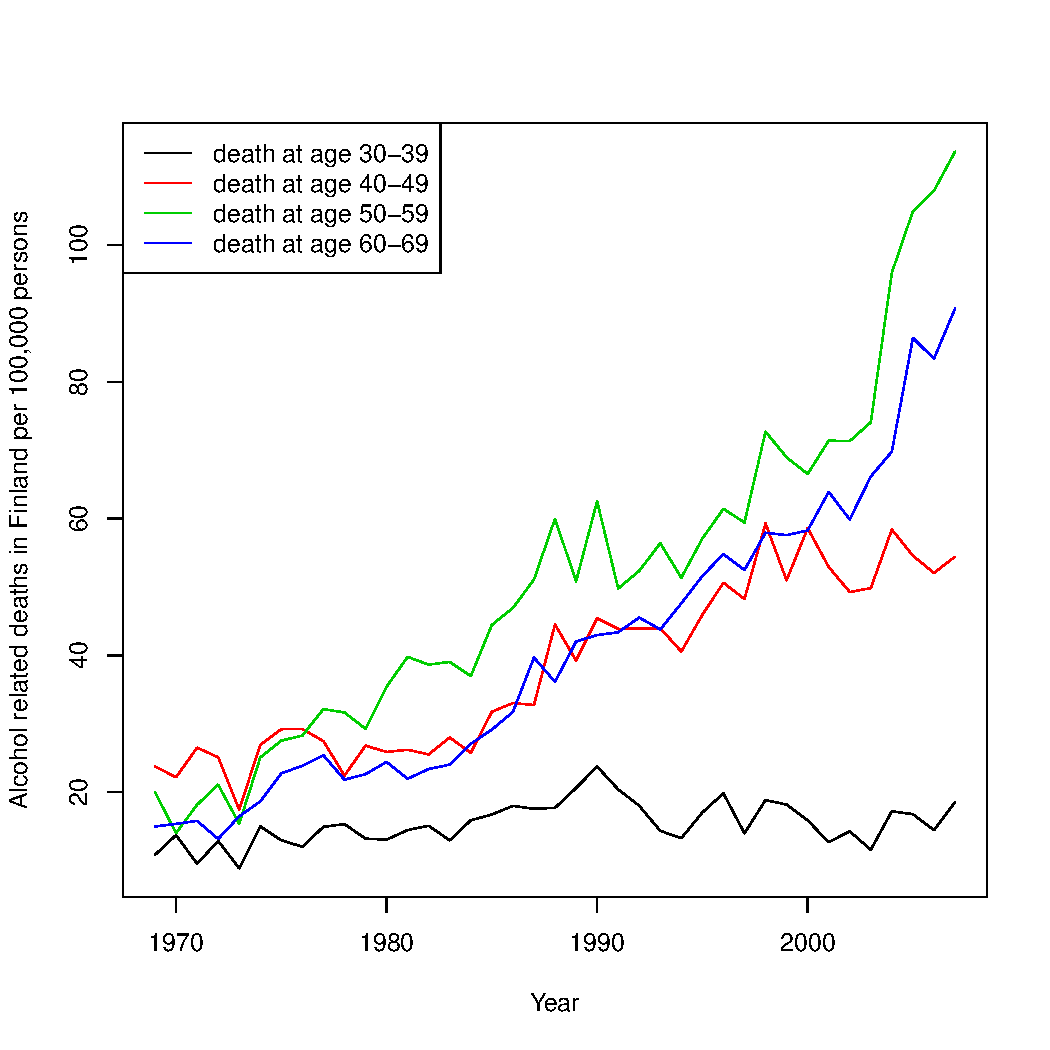
\includegraphics[width=\linewidth]{figure/alcoholPlot1} \caption[Alcohol related deaths per 100,000 persons in Finland in 1969--2007]{Alcohol related deaths per 100,000 persons in Finland in 1969--2007.\label{fig:alcoholPlot1}}
\end{figure}


\end{knitrout}

Natural distributional assumption for modelling counts is a Poisson distribution. Based on the time series plot, we can think of several candidates for capturing the time series aspects of the series. One could try for example an ARIMA model or a structural time series model such as local level or local linear trend. These are closely related, but I feel that the latter models are more easily interpretable so I will use structural time series approach.

Here I choose a multivariate Poisson model 

\begin{equation*}\label{alcohol}
\begin{aligned}
p(y_t|\theta_t) &= Poisson(u_t e^{\theta_t}), \quad u_t = \textrm{population}_t,\\
\theta_t &= \mu_t + \epsilon_t, \quad \epsilon_t \sim N(0, Q_{\textrm{noise}}),\\
\mu_{t+1} &= \mu_t + \nu_t + \xi_t, \quad \xi_t \sim N(0, Q_{\textrm{level}}), \\ 
\nu_{t+1} &= \nu_t,
\end{aligned}
\end{equation*}

where $\mu_t$ is the random walk with drift component, $\nu_t$ is a constant slope and $\epsilon_t$ is an additional white noise component which captures the extra variation of the series. I make no restrictions for the covariance structures of the level or the noise component. Note that the random walk with drift is a special case of local linear trend model where the covariance structure of the slope term is set to zero.


We estimate the model parameters first without simulation, and then using those estimates as initial values run the estimation procedure again with importance sampling. In this case, the results obtained from the importance sampling step are practically identical with the ones obtained from the initial step.

\begin{knitrout}
\definecolor{shadecolor}{rgb}{0.969, 0.969, 0.969}\color{fgcolor}\begin{kframe}
\begin{alltt}
\hlcom{# remove the last observations}
\hlstd{alcoholPred} \hlkwb{<-} \hlkwd{window}\hlstd{(alcohol,} \hlkwc{start} \hlstd{=} \hlnum{1969}\hlstd{,} \hlkwc{end} \hlstd{=} \hlnum{2007}\hlstd{)}

\hlstd{model} \hlkwb{<-} \hlkwd{SSModel}\hlstd{(alcoholPred[,}\hlnum{1}\hlopt{:}\hlnum{4}\hlstd{]} \hlopt{~}
                   \hlkwd{SSMtrend}\hlstd{(}\hlnum{2}\hlstd{,} \hlkwc{Q} \hlstd{=} \hlkwd{list}\hlstd{(}\hlkwd{matrix}\hlstd{(}\hlnum{NA}\hlstd{,}\hlnum{4}\hlstd{,}\hlnum{4}\hlstd{),} \hlkwd{matrix}\hlstd{(}\hlnum{0}\hlstd{,}\hlnum{4}\hlstd{,}\hlnum{4}\hlstd{)))} \hlopt{+}
                   \hlkwd{SSMcustom}\hlstd{(}\hlkwc{Z} \hlstd{=} \hlkwd{diag}\hlstd{(}\hlnum{1}\hlstd{,}\hlnum{4}\hlstd{),} \hlkwc{T} \hlstd{=} \hlkwd{diag}\hlstd{(}\hlnum{0}\hlstd{,}\hlnum{4}\hlstd{),}
                             \hlkwc{Q} \hlstd{=} \hlkwd{matrix}\hlstd{(}\hlnum{NA}\hlstd{,}\hlnum{4}\hlstd{,}\hlnum{4}\hlstd{),} \hlkwc{P1} \hlstd{=} \hlkwd{matrix}\hlstd{(}\hlnum{NA}\hlstd{,}\hlnum{4}\hlstd{,}\hlnum{4}\hlstd{)),}
                 \hlkwc{distribution} \hlstd{=} \hlstr{"poisson"}\hlstd{,} \hlkwc{u} \hlstd{= alcoholPred[,}\hlnum{5}\hlopt{:}\hlnum{8}\hlstd{])}

\hlcom{# Model updating function for fitSSM}
\hlstd{updatefn} \hlkwb{<-} \hlkwa{function}\hlstd{(}\hlkwc{pars}\hlstd{,} \hlkwc{model}\hlstd{,} \hlkwc{...}\hlstd{)\{}
  \hlstd{Q} \hlkwb{<-} \hlkwd{diag}\hlstd{(}\hlkwd{exp}\hlstd{(pars[}\hlnum{1}\hlopt{:}\hlnum{4}\hlstd{]))}
  \hlstd{Q[}\hlkwd{upper.tri}\hlstd{(Q)]} \hlkwb{<-} \hlstd{pars[}\hlnum{5}\hlopt{:}\hlnum{10}\hlstd{]}
  \hlstd{model[}\hlstr{"Q"}\hlstd{,}\hlkwc{etas}\hlstd{=}\hlstr{"level"}\hlstd{]} \hlkwb{<-} \hlkwd{crossprod}\hlstd{(Q)}
  \hlstd{Q} \hlkwb{<-} \hlkwd{diag}\hlstd{(}\hlkwd{exp}\hlstd{(pars[}\hlnum{11}\hlopt{:}\hlnum{14}\hlstd{]))}
  \hlstd{Q[}\hlkwd{upper.tri}\hlstd{(Q)]} \hlkwb{<-} \hlstd{pars[}\hlnum{15}\hlopt{:}\hlnum{20}\hlstd{]}
  \hlstd{model[}\hlstr{"Q"}\hlstd{,}\hlkwc{etas}\hlstd{=}\hlnum{9}\hlopt{:}\hlnum{12}\hlstd{]} \hlkwb{<-} \hlstd{model[}\hlstr{"P1"}\hlstd{,}\hlkwc{states}\hlstd{=}\hlnum{9}\hlopt{:}\hlnum{12}\hlstd{]} \hlkwb{<-} \hlkwd{crossprod}\hlstd{(Q)}
  \hlstd{model}
\hlstd{\}}
\hlcom{# Initial the covariance structure of the random walks and extra noise}
\hlcom{# theta = log(intensity) = log(y/u)}
\hlcom{# covariance matrices are parameterized via log-Cholesky in fitSSM}
\hlstd{init} \hlkwb{<-} \hlkwd{chol}\hlstd{(}\hlkwd{cov}\hlstd{(}\hlkwd{log}\hlstd{(alcoholPred[,}\hlnum{1}\hlopt{:}\hlnum{4}\hlstd{]}\hlopt{/}\hlstd{alcoholPred[,}\hlnum{5}\hlopt{:}\hlnum{8}\hlstd{]))}\hlopt{/}\hlnum{10}\hlstd{)}

\hlstd{fitinit} \hlkwb{<-} \hlkwd{fitSSM}\hlstd{(model,} \hlkwc{updatefn} \hlstd{= updatefn,}
                  \hlkwc{inits} \hlstd{=} \hlkwd{rep}\hlstd{(}\hlkwd{c}\hlstd{(}\hlkwd{log}\hlstd{(}\hlkwd{diag}\hlstd{(init)), init[}\hlkwd{upper.tri}\hlstd{(init)]),}\hlnum{2}\hlstd{),}
                  \hlkwc{method} \hlstd{=} \hlstr{"BFGS"}\hlstd{)}
\hlcom{# Now with simulation}
\hlstd{fit}\hlkwb{<-}\hlkwd{fitSSM}\hlstd{(model,} \hlkwc{updatefn} \hlstd{= updatefn,}
            \hlkwc{inits} \hlstd{= fitinit}\hlopt{$}\hlstd{optim.out}\hlopt{$}\hlstd{par,} \hlkwc{method} \hlstd{=} \hlstr{"BFGS"}\hlstd{,} \hlkwc{nsim} \hlstd{=} \hlnum{250}\hlstd{)}
\hlstd{varcor} \hlkwb{<-} \hlstd{fit}\hlopt{$}\hlstd{model[}\hlstr{"Q"}\hlstd{,} \hlkwc{etas} \hlstd{=} \hlstr{"level"}\hlstd{]}
\hlstd{varcor[}\hlkwd{upper.tri}\hlstd{(varcor)]} \hlkwb{<-} \hlkwd{cov2cor}\hlstd{(varcor)[}\hlkwd{upper.tri}\hlstd{(varcor)]}
\hlkwd{print}\hlstd{(varcor,}\hlkwc{digits}\hlstd{=}\hlnum{2}\hlstd{)} \hlcom{#local level component}
\end{alltt}
\begin{verbatim}
##        [,1]    [,2]   [,3]  [,4]
## [1,] 0.0074 0.66022 0.8062 0.856
## [2,] 0.0028 0.00239 0.1654 0.711
## [3,] 0.0040 0.00047 0.0034 0.755
## [4,] 0.0033 0.00156 0.0020 0.002
\end{verbatim}
\begin{alltt}
\hlstd{varcor} \hlkwb{<-} \hlstd{fit}\hlopt{$}\hlstd{model[}\hlstr{"Q"}\hlstd{,} \hlkwc{etas} \hlstd{=} \hlstr{"custom"}\hlstd{]}
\hlstd{varcor[}\hlkwd{upper.tri}\hlstd{(varcor)]} \hlkwb{<-} \hlkwd{cov2cor}\hlstd{(varcor)[}\hlkwd{upper.tri}\hlstd{(varcor)]}
\hlkwd{print}\hlstd{(varcor,}\hlkwc{digits}\hlstd{=}\hlnum{2}\hlstd{)} \hlcom{#local level component #extra noise component}
\end{alltt}
\begin{verbatim}
##         [,1]    [,2]    [,3]    [,4]
## [1,] 0.00537 0.73118 0.75627 8.0e-01
## [2,] 0.00315 0.00346 0.99924 9.9e-01
## [3,] 0.00295 0.00313 0.00283 1.0e+00
## [4,] 0.00043 0.00043 0.00039 5.4e-05
\end{verbatim}
\begin{alltt}
\hlopt{-}\hlstd{fitinit}\hlopt{$}\hlstd{optim.out}\hlopt{$}\hlstd{val} \hlcom{#log-likelihood without simulation}
\end{alltt}
\begin{verbatim}
## [1] -704.8
\end{verbatim}
\begin{alltt}
\hlopt{-}\hlstd{fit}\hlopt{$}\hlstd{optim.out}\hlopt{$}\hlstd{val}     \hlcom{#log-likelihood with simulation  }
\end{alltt}
\begin{verbatim}
## [1] -704.8
\end{verbatim}
\end{kframe}
\end{knitrout}

Parameter estimation of state space model is often a difficult task, as the likelihood surface contains multiple maxima, thus making the optimization problem highly dependent on the initial values. Often the unknown parameters are related to the unobserved latent states such as the covariance matrix in this example, without much a priori knowledge. Therefore, it is challenging to guess good initial values especially in more complex settings and multiple initial value configurations possibly with several different type of optimization routines is recommended before one can be reasonably sure that proper optimum is found. Here we use the covariance matrix of the observed series as initial values for the covariance structures.

Another issue in case of non-Gaussian models is the fact that the likelihood computation is based on iterative procedure which is stopped using some stopping criteria (such as relative change of log-likelihood), so the function actually contains some noise. This in turn affects the gradient computations in BFGS and can in theory give unreliable results. Using derivative free method like Nelder-Mead is therefore sometimes recommended. On the other hand BFGS is usually much faster than Nelder-Mead and thus I prefer to try first BFGS at least in preliminary analysis.

Using function \code{KFS} we can compute the smoothed estimates of states:

\begin{knitrout}
\definecolor{shadecolor}{rgb}{0.969, 0.969, 0.969}\color{fgcolor}\begin{kframe}
\begin{alltt}
\hlstd{out} \hlkwb{<-} \hlkwd{KFS}\hlstd{(fit}\hlopt{$}\hlstd{model,} \hlkwc{nsim} \hlstd{=} \hlnum{1000}\hlstd{)}
\hlstd{out}
\end{alltt}
\begin{verbatim}
## 
##  Smoothed values of states and standard errors at time n = 39:
##                           Estimate   Std. Error
## level.death at age 30-39   2.855916   0.078437 
## slope.death at age 30-39   0.010714   0.013714 
## level.death at age 40-49   4.031312   0.042376 
## slope.death at age 40-49   0.023719   0.007632 
## level.death at age 50-59   4.757803   0.039830 
## slope.death at age 50-59   0.050371   0.009585 
## level.death at age 60-69   4.493837   0.033290 
## slope.death at age 60-69   0.048239   0.007209 
## custom1                   -0.000402   0.060395 
## custom2                   -0.019549   0.040885 
## custom3                   -0.016949   0.037024 
## custom4                   -0.002134   0.005143
\end{verbatim}
\end{kframe}
\end{knitrout}

From the output of \code{KFS} we see that the slope term is not significant in the first age group. For time-varying states we can easily plot the estimated level and noise components, which shows clear trends in three age groups and highly correlated additional variation in all groups:

\begin{knitrout}
\definecolor{shadecolor}{rgb}{0.969, 0.969, 0.969}\color{fgcolor}\begin{kframe}
\begin{alltt}
\hlkwd{plot}\hlstd{(}\hlkwd{coef}\hlstd{(out,}\hlkwc{states}\hlstd{=}\hlkwd{c}\hlstd{(}\hlstr{"level"}\hlstd{,}\hlstr{"custom"}\hlstd{)),}
     \hlkwc{main} \hlstd{=} \hlstr{"Smoothed states"}\hlstd{,} \hlkwc{yax.flip}\hlstd{=}\hlnum{TRUE}\hlstd{)}
\end{alltt}
\end{kframe}\begin{figure}[!ht]

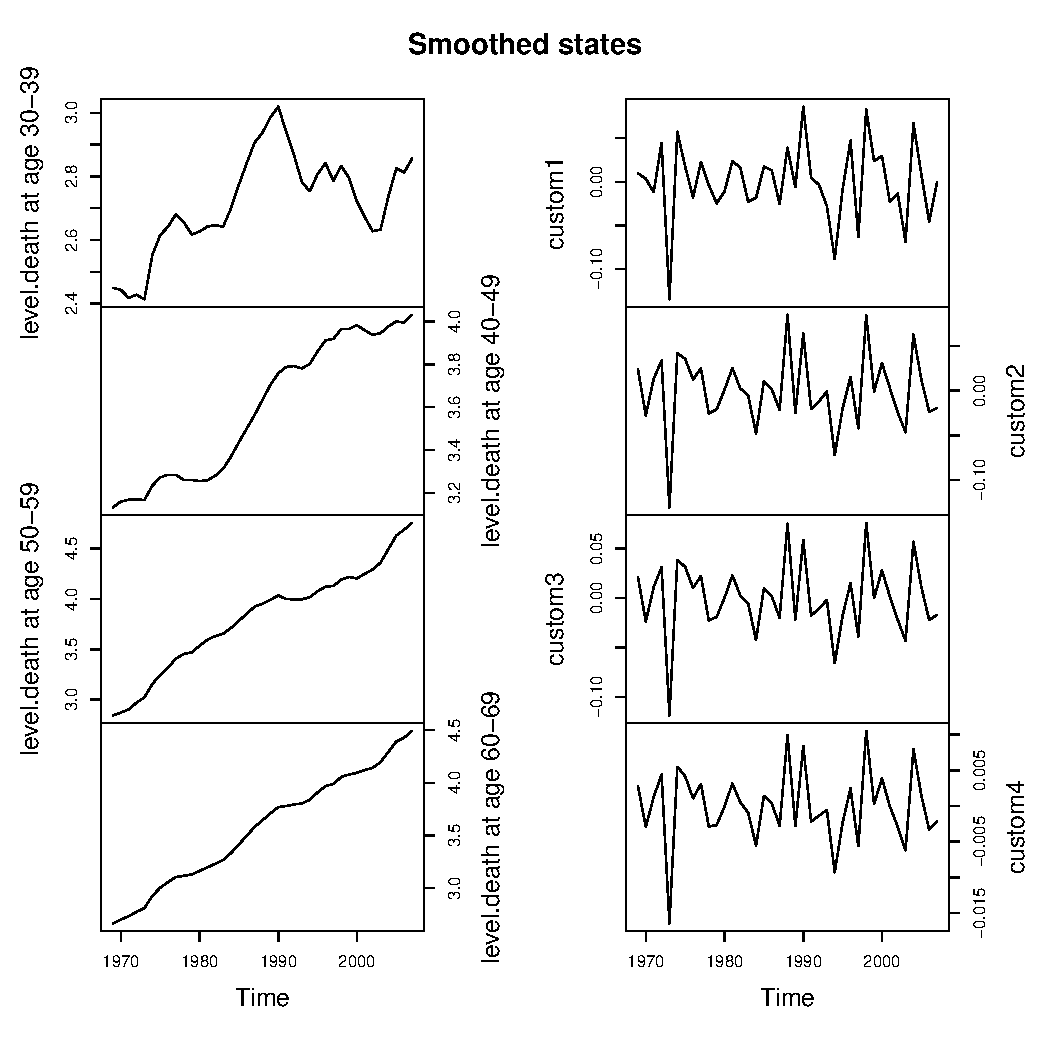
\includegraphics[width=\linewidth]{figure/states} \caption[Smoothed level and white noise components]{Smoothed level and white noise components.\label{fig:states}}
\end{figure}


\end{knitrout}

Note the large drop in noise component which relates to possible outlier in 1973 of the mortality series. As an illustration of model diagnostics, we compute recursive residuals for our model and check whether there is autocorrelation left in the residuals (Figure \ref{fig:diagnostics1}).

\begin{knitrout}
\definecolor{shadecolor}{rgb}{0.969, 0.969, 0.969}\color{fgcolor}\begin{kframe}
\begin{alltt}
\hlstd{res} \hlkwb{<-} \hlkwd{rstandard}\hlstd{(}\hlkwd{KFS}\hlstd{(fit}\hlopt{$}\hlstd{model,} \hlkwc{filtering} \hlstd{=} \hlstr{"mean"}\hlstd{,}
                     \hlkwc{smoothing} \hlstd{=} \hlstr{"none"}\hlstd{,} \hlkwc{nsim} \hlstd{=} \hlnum{1000}\hlstd{))}
\hlkwd{acf}\hlstd{(res,} \hlkwc{na.action} \hlstd{= na.pass)}
\end{alltt}
\end{kframe}\begin{figure}[!ht]

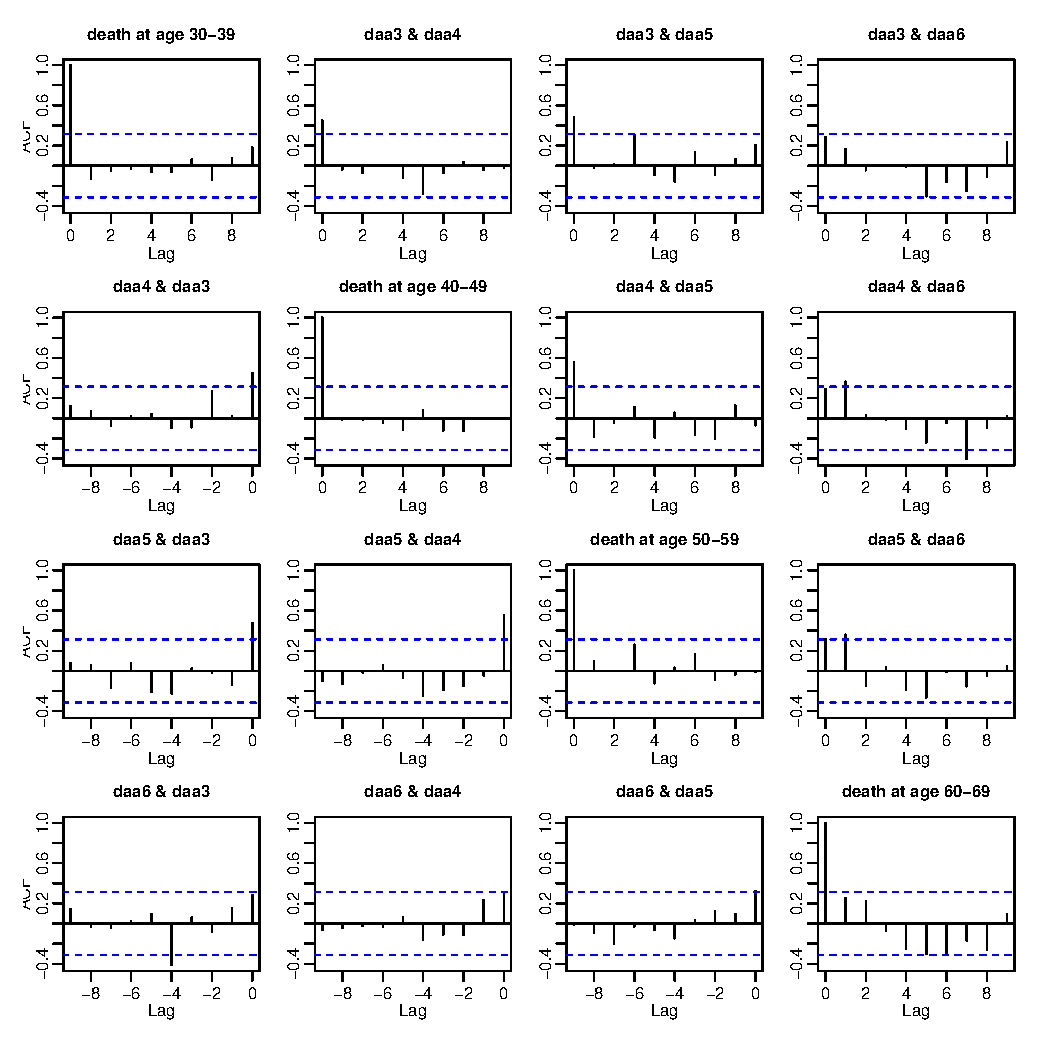
\includegraphics[width=\linewidth]{figure/diagnostics1} \caption[Autocorrelations and cross-correlations of recursive residuals]{Autocorrelations and cross-correlations of recursive residuals.\label{fig:diagnostics1}}
\end{figure}


\end{knitrout}

We see occasional lagged cross-correlation between the residuals, but overall we can be relatively satisfied with our model. 

We can now predict the intensity $e^{\theta_t}$ of alcohol related deaths per 100,000 persons for each age group for years 2008--2015 using our estimated model. As our model is time varying (\code{u} varies), we need to provide the model for the future observations via \code{newdata} argument. In this case we can use \code{SSMcustom} function and provide all the necessary system matrices as once, together with constant \code{u=1} (our signal $\theta$ is already scaled properly as the original $u_t$ was the population per 100,000 persons).

\begin{knitrout}
\definecolor{shadecolor}{rgb}{0.969, 0.969, 0.969}\color{fgcolor}\begin{kframe}
\begin{alltt}
\hlstd{pred}\hlkwb{<-}\hlkwd{predict}\hlstd{(fit}\hlopt{$}\hlstd{model,} \hlkwc{newdata} \hlstd{=}
                \hlkwd{SSModel}\hlstd{(}\hlkwd{ts}\hlstd{(}\hlkwd{matrix}\hlstd{(}\hlnum{NA}\hlstd{,}\hlnum{6}\hlstd{,}\hlnum{4}\hlstd{),} \hlkwc{start} \hlstd{=} \hlnum{2008}\hlstd{)} \hlopt{~ -}\hlnum{1}
                        \hlopt{+} \hlkwd{SSMcustom}\hlstd{(}\hlkwc{Z} \hlstd{= fit}\hlopt{$}\hlstd{model}\hlopt{$}\hlstd{Z,} \hlkwc{T} \hlstd{= fit}\hlopt{$}\hlstd{model}\hlopt{$}\hlstd{T,}
                                    \hlkwc{R} \hlstd{= fit}\hlopt{$}\hlstd{model}\hlopt{$}\hlstd{R,} \hlkwc{Q} \hlstd{= fit}\hlopt{$}\hlstd{model}\hlopt{$}\hlstd{Q),} \hlkwc{u} \hlstd{=} \hlnum{1}\hlstd{,}
                        \hlkwc{distribution}\hlstd{=} \hlstr{"poisson"}\hlstd{),}
              \hlkwc{interval} \hlstd{=} \hlstr{"confidence"}\hlstd{,} \hlkwc{nsim} \hlstd{=} \hlnum{10000}\hlstd{)}
\end{alltt}
\end{kframe}
\end{knitrout}
\begin{knitrout}
\definecolor{shadecolor}{rgb}{0.969, 0.969, 0.969}\color{fgcolor}\begin{kframe}
\begin{alltt}
\hlstd{trend} \hlkwb{<-} \hlkwd{exp}\hlstd{(}\hlkwd{signal}\hlstd{(out,} \hlstr{"trend"}\hlstd{)}\hlopt{$}\hlstd{signal)}
\hlkwd{par}\hlstd{(}\hlkwc{mfrow} \hlstd{=} \hlkwd{c}\hlstd{(}\hlnum{2}\hlstd{,}\hlnum{2}\hlstd{),} \hlkwc{mar} \hlstd{=} \hlkwd{c}\hlstd{(}\hlnum{2}\hlstd{,}\hlnum{2}\hlstd{,}\hlnum{2}\hlstd{,}\hlnum{2}\hlstd{)} \hlopt{+} \hlnum{0.1}\hlstd{,} \hlkwc{oma} \hlstd{=} \hlkwd{c}\hlstd{(}\hlnum{2}\hlstd{,}\hlnum{2}\hlstd{,}\hlnum{0}\hlstd{,}\hlnum{0}\hlstd{))}
\hlkwa{for}\hlstd{(i} \hlkwa{in} \hlnum{1}\hlopt{:}\hlnum{4}\hlstd{)}
  \hlkwd{ts.plot}\hlstd{(alcohol[,i]}\hlopt{/}\hlstd{alcohol[,}\hlnum{4}\hlopt{+}\hlstd{i],}
          \hlstd{trend[,i],}
          \hlstd{pred[[i]],}
          \hlkwc{col} \hlstd{=} \hlkwd{c}\hlstd{(}\hlnum{1}\hlstd{,}\hlnum{2}\hlstd{,}\hlkwd{rep}\hlstd{(}\hlnum{3}\hlstd{,}\hlnum{3}\hlstd{)),} \hlkwc{xlab} \hlstd{=} \hlkwa{NULL}\hlstd{,} \hlkwc{ylab} \hlstd{=} \hlkwa{NULL}\hlstd{,}
          \hlkwc{main} \hlstd{=} \hlkwd{colnames}\hlstd{(alcohol)[i])}
\hlkwd{mtext}\hlstd{(}\hlstr{"Number of alcohol related deaths per 100,000 persons in Finland"}\hlstd{,}
      \hlkwc{side} \hlstd{=} \hlnum{2}\hlstd{,} \hlkwc{outer} \hlstd{=} \hlnum{TRUE}\hlstd{)}
\hlkwd{mtext}\hlstd{(}\hlstr{"Year"}\hlstd{,}\hlkwc{side}\hlstd{=}\hlnum{1}\hlstd{,}\hlkwc{outer}\hlstd{=}\hlnum{TRUE}\hlstd{)}
\end{alltt}
\end{kframe}\begin{figure}[!ht]

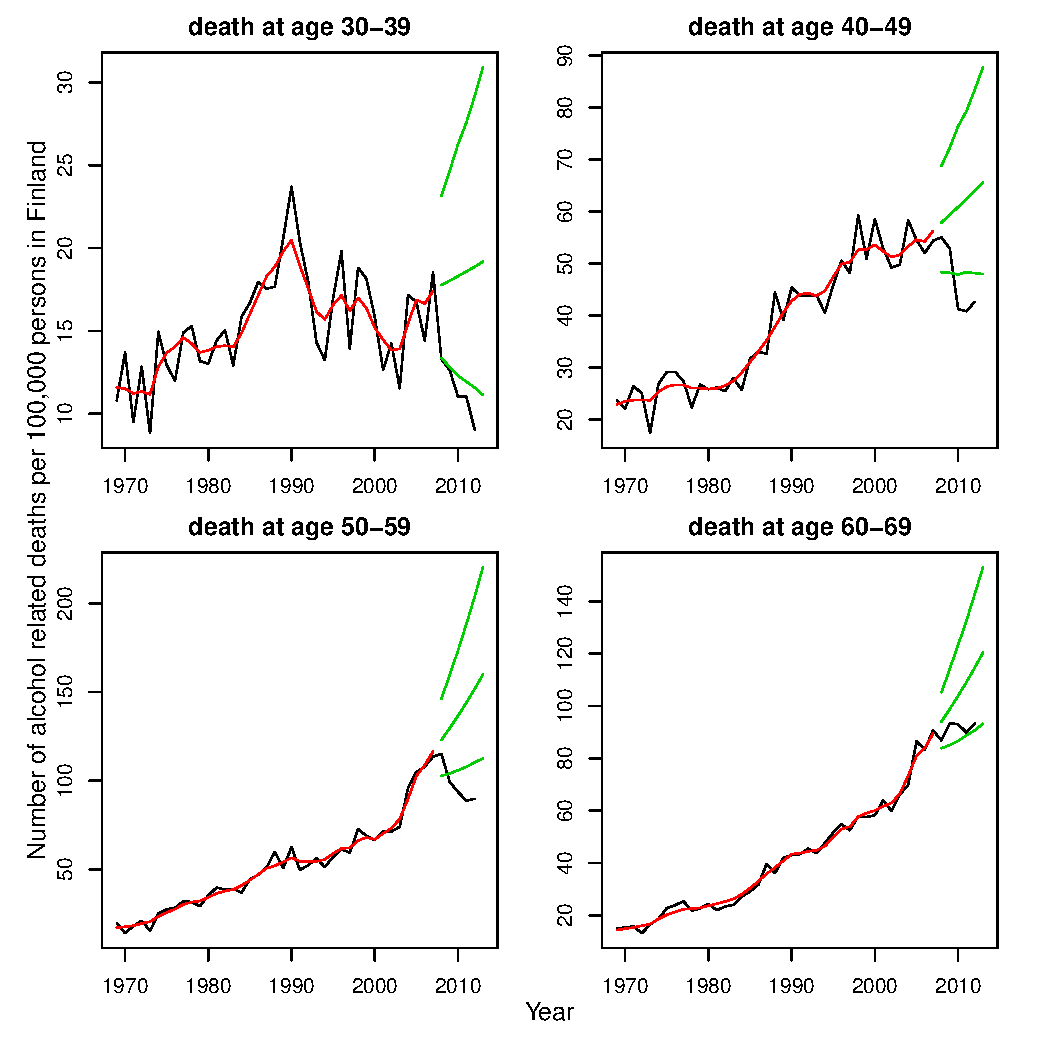
\includegraphics[width=\linewidth]{figure/predictplot} \caption[Observed number of alcohol related deaths per 100,000 persons in Finland (black), fitted values (red) and intensity predictions for years 2008--2012 together with 95\% prediction intervals (green)]{Observed number of alcohol related deaths per 100,000 persons in Finland (black), fitted values (red) and intensity predictions for years 2008--2012 together with 95\% prediction intervals (green).\label{fig:predictplot}}
\end{figure}


\end{knitrout}

Figure \ref{fig:predictplot} shows the observed deaths, smoothed trends for 1969--2007, and intensity predictions for 2008--2012 together with 95\% prediction intervals for intensity. When we compare our predictions to true observations, we see that in reality the number of deaths slightly increased in the oldest age group (ages 60--69), whereas in other age they decreased substantially during the forecasting period. This is partly explained by the fact that during this period the total alcohol consumption decreased almost monotonically, which in turn might have been caused by the increase in taxation of alcohol in 2008, 2009 and 2012.

% \section[Comparison to INLA]{Comparison to \pkg{INLA}}\label{comparison}
% 
% I will now shortly compare \pkg{KFAS} and \pkg{INLA}, which is an \proglang{R} package for approximate Bayesian inference for latent Gaussian models by using integrated nested Laplace approximation \citep{Rue}.
% 
% As an illustration, we reanalyze the salmonella data analyzed by \citet{Margolin} which is available from \pkg{INLA}. The data consists of the number of revertant colonies of TA98 Salmonella with different doses of quinoline. We model the number of colonies as a Poisson GLMM with two explanatory variables and a random intercept term which tries to capture the overdispersion in the data. The codes for inference with \pkg{INLA} used here can be found from \url{http://www.r-inla.org/examples/volume-1/code-for-salm-example}.
% 
% <<'salmonellaINLA'>>=
% suppressWarnings(library("INLA",quietly = TRUE))
% data("Salm")
% mod.salm <- inla(y ~ log(dose+10) + dose + 
%                    f(rand, model = "iid", param = c(0.001,0.001)),
%                  family = "poisson", data = Salm)
% ## improved estimation of the hyperparameters
% h.salm <- inla.hyperpar(mod.salm)
% @
% 
% There are two ways to define the random intercept component in \pkg{KFAS}. The first one uses the \code{SSMregression} function and constructs a factor with 18 levels (one for each case) with non-diffuse initial variance $\sigma^2$. This gives 18 identically distributed time-invariant states where each state correspond to random effect of one observation. Another option would be to use \code{SSMcustom} function and define just one time-varying state as \code{SSMcustom(Z = 1, T = 0,  R = 1, Q = sigma2, a1 = 0, P1 = sigma2,  P1inf = 0)}. Both approaches give identical results. However, for large data the former approach is less efficient as the number of states depends on the number of observations. Nevertheless, we use the former approach here for illustration.
% 
% <<'salmonellaKFAS'>>=
% Salm$rand<-as.factor(Salm$rand)
% model <- SSModel(y ~ log(dose+10) + dose + 
%                    SSMregression(~ -1 + rand, P1 = diag(NA,18), 
%                                  remove.intercept = FALSE),
%                  data = Salm, distribution = "poisson")
% 
% updatefn<-function(pars,model,...){
%   diag(model["P1", states = 4:21]) <- exp(pars)
%   model  
% }
% 
% fit <- fitSSM(model, updatefn = updatefn, inits = -3, 
%               method = "BFGS", nsim = 1000)
% @
% 
% <<'salmonellaResults'>>=
% out<-KFS(fit$model,nsim=1000)
% out
% h.salm$summary.fixed[,1:2]
% h.salm$summary.random$rand[,2:3]
% 1/h.salm$summary.hyper[1]
% fit$model["P1", states = 4]
% @
% 
% Although \pkg{INLA} uses Bayesian approach which takes account the parameter estimation uncertainty, the results from \pkg{INLA} and \pkg{KFAS} are practically same, even with such a small data. Kalman filtering with diffuse initialization still takes account the uncertainty of the estimation of regression coefficients, so the differences here are related to the estimation of hyperparameter $\sigma^2$, which is estimated as precision $1/\sigma^2$ by \pkg{INLA}. The estimate of $\sigma^2$ by \pkg{KFAS} is signif(fit$model["P1", states = 4],2) whereas \pkg{INLA} gives $\sigma^2=signif(1/h.salm$summary.hyper[1],2)$.
% 
% As \pkg{INLA} and \pkg{KFAS} are based on different (although related) theoretical framework, the extensive study of their performances in terms of computational efficiency and accuracy of results is somewhat pointless. Nevertheless, some remarks can be made. I feel that the biggest advantage of \pkg{INLA} is the Bayesian framework which allows us to take account the parameter uncertainty in predictions and other inference. On the other hand, the computational burden related to the numerical integration over the hyperparameters can become infeasible as the number of hyperparameters increase. It is not uncommon to have a time series model with tens (or even hundreds) of parameters (such as multivariate structural time series or dynamic factor models). Of course these same models cause problems also to the maximum likelihood estimation, as noted in the previous section. Also the Bayesian approach eliminates the need for defining good initial values for the maximum likelihood estimation but the problem transforms into defining good priors for the same hyperparameters which again is a non-trivial task in practice.

\section{Discussion}

State space models offers tools for solving a large class of statistical problems. Here I introduced an R package \pkg{KFAS} for linear state space modelling where the observations are from an exponential family. With such a general framework, different aspects of the modelling need to be taken into account. Therefore the focus of the package has been to provide reliable and relatively fast tools for multiple inference problems, such as maximum likelihood estimation, filtering, smoothing and simulation. Compared to the early versions of \pkg{KFAS}, constructing a state space model with simple components is now possible without explicit definition of the system matrices by using the auxiliary functions and symbolic descriptions with the help of formula objects, which should greatly ease the use of the package.

Currently all the time consuming parts of \pkg{KFAS} are written in \proglang{Fortran}, which makes it relatively fast, given the general nature of problems \pkg{KFAS} can handle. Still, converting the package to \proglang{C++} and \code{S4} classes with help of \pkg{Rcpp} \citep{RcppA,RcppB} could result potential improvements in terms of memory management, scalability and maintenance.

\section*{Acknowledgments}

The author wishes to thank Jukka Nyblom and Patricia Menendez for the valuable comments and suggestions regarding the paper and the package. Author is also grateful for the financial support from Emil Aaltonen's Foundation.

\clearpage
\newpage
\appendix
\section{Appendix: Filtering and smoothing recursions}\label{appendix}

The following formulas summarize the Kalman filtering and smoothing formulas for diffuse and sequential case and  are based on \citet{DK2001} and related articles. The original formulas are somewhat scattered between the references with slightly different notations. Therefore I have collected the equations used in \pkg{KFAS} to this Appendix.
\subsection{Filtering}
Denote
\begin{equation*}
\begin{aligned}
a_{t+1} &= \E(\alpha_{t+1}|y_t,\ldots,y_1) \quad \textrm{and}  \\
P_{t+1} &= \VAR(\alpha_{t+1}|y_t,\ldots,y_1).
\end{aligned}
\end{equation*}
The Kalman filter recursions for the general Gaussian model of form \eqref{ssgeneral} are
\begin{equation*}
\begin{aligned}
v_t &= y_t - Z_t a_t \\
F_t &= Z_t P_t Z_t^\top + H_t \\
K_t &= P_t Z_t^\top \\
a_{t+1} &= T_t (a_t + K_t F^{-1}_t v_t) \\
P_{t+1} &= T_t (P_t -K_tF^{-1}_tK_t^\top)T_t^\top + R_t Q_t R_t,
\end{aligned}
\end{equation*}

For the univariate approach, the filtering equations are
\begin{equation*}
\begin{aligned}
v_{t,i} &= y_{t,i} - Z_{t,i} a_{t,i} \\
F_{t,i} &= Z_{t,i} P_{t,i} Z_{t,i}^\top + \sigma^2_{t,i} \\
K_{t,i} &= P_{t,i} Z_{t,i}^\top \\
a_{t,i+1} &= a_{t,i} + K_{t,i}F_{t,i}^{-1} v_{t,i} \\
P_{t,i+1} &= P_{t,i} -K_{t,i}K^\top_{t,i}F_{t,i}^{-1}\\
a_{t+1,1} &= T_t a_{t,p_t+1}\\
P_{t+1,1} &= T_t P_{t,p_t+1} T_t^\top + R_t Q_t R_t, 
\end{aligned}
\end{equation*}
for $t=1,\ldots,n$ and  $i=1,\ldots,p_t$, where $v_{t,i}$ and $F_{t,i}$ are
scalars, $K_{t,i}$ is a column vector and $\sigma^2_{t,i}$ is the $i$th diagonal
element of $H_t$. It is possible that $F_{t,i}=0$, which case $a_{t,i+1} =
a_{t,i}$, $P_{t,i+1} = P_{t,i}$, and $v_{t,i}$ is computed as usual.  

The diffuse filtering equations for univariate approach are
\begin{equation*}
\begin{aligned}
v_{t,i} &= y_{t,i} - Z_{t,i} a_{t,i} \\
F_{\ast,t,i} &= Z_{t,i} P_{\ast,t,i} Z_{t,i}^\top + \sigma^2_{t,i} \\
F_{\infty,t,i} &= Z_{t,i} P_{\infty,t,i} Z_{t,i}^\top \\
K_{\ast,t,i} &= P_{\ast,t,i} Z_{t,i}^\top \\
K_{\infty,t,i} &= P_{\infty,t,i} Z_{t,i}^\top,
\end{aligned}
\end{equation*}

and

\begin{equation*}
\begin{aligned}
a_{t,i+1} &= a_{t,i} + K_{\infty,t,i} v_{t,i}F_{\infty,t,i}^{-1} \\
P_{\ast,t,i+1} &= P_{\ast,t,i}
+K_{\infty,t,i}K^\top_{\infty,t,i}F_{\ast,t,i}F_{\infty,t,i}^{-2}
-(K_{\ast,t,i}K^\top_{\infty,t,i}+K_{\ast,t,i}K^\top_{\infty,t,i})F_{\infty,t,i}^{-1}\\
P_{\infty,t,i+1} &= P_{\infty,t,i}
-K_{\infty,t,i}K^\top_{\infty,t,i}F_{\infty,t,i}^{-1}\\
\end{aligned} 
\end{equation*}

if $F_{\infty,t,i}>0$, and

\begin{equation*} 
\begin{aligned}
a_{t,i+1} &= a_{t,i} + K_{\ast,t,i} v_{t,i}F_{\ast,t,i}^{-1} \\
P_{\ast,t,i+1} &= P_{\ast,t,i} -K_{\ast,t,i}K^\top_{\ast,t,i}F_{\ast,t,i}^{-1}\\
P_{\infty,t,i+1} &= P_{\infty,t,i},\\
\end{aligned} 
\end{equation*}

if $F_{\infty,t,i}=0$. The transition equations from $t$ to $t+1$ are

\begin{equation*} 
\begin{aligned}
a_{t+1,1} &= T_t a_{t,p_t+1}\\
P_{\ast,t+1,1} &= T_t P_{\ast,t,p_t+1} T_t^\top + R_t Q_t R_t\\
P_{\infty,t+1,1} &= T_t P_{\infty,t,p_t+1} T_t^\top. 
\end{aligned}
\end{equation*}


\subsection{Smoothing}
Denote
\begin{equation*} 
\begin{aligned}
\hat\alpha_{t} &= \E(\alpha_{t}|y_n,\ldots,y_1) \quad \textrm{and}  \\
V_{t} &= \VAR(\alpha_{t}|y_n,\ldots,y_1).
\end{aligned} 
\end{equation*}

The smoothing algorithms of \pkg{KFAS} are based on the following recursions:

\begin{equation*} 
\begin{aligned}
r_{t,i-1} &= Z_{t,i}^\top v_{t,i}F_{t,i}^{-1} + L_{t,i}^\top r_{t,i}, \\
r_{t-1,p_t} &= T_{t-1}^\top r_{t,0},\\
N_{t,i-1} &= Z_{t,i}^\top Z_{t,i}F_{t,i}^{-1} +L_{t,i}^\top N_{t,i}L_{t,i},\\
N_{t-1,p_t} &= T_{t-1}^\top N_{t,0}T_{t-1},\\
L_{t,i} &= I - K_{t,i}Z_{t,i}^\top F_{t,i}^{-1},
\end{aligned} 
\end{equation*}

for $t=n,\ldots,1$ and  $i=p_t,\ldots,1$, with $r_{n,p_n}=0$ and $N_{n,p_n}=0$.
From these recursions, we get state smoothing recursions
\begin{equation*} 
\begin{aligned}
\hat\alpha_{t} &= a_{t,1} + P_{t,1}r_{t,0}\\
V_{t} &= P_{t,1}-P_{t,1}N_{t,0}P_{t,1},
\end{aligned} 
\end{equation*}

and disturbance smoothing recursions

\begin{equation*} 
\begin{aligned}
\hat \epsilon_{t,i} &= \sigma^2_{t,i}F_{t,i}^{-1}(v_{t,i} -K_{t,i}^\top r_{t,i}),\\
\VAR(\hat \epsilon_{t,i}) &= \sigma^2_{t,i} -
\sigma^4_{t,i}(F_{t,i}^{-1} -K_{t,i}^\top N_{t,i}K_{t,i}F_{t,i}^{-2}),\\
\hat \eta_{t} &= Q_tR_t^\top r_{t,0},\\
\VAR(\hat \eta_{t,i}) &= Q_tR^\top_t N_{t,0}R_tQ_t.
\end{aligned} 
\end{equation*}
The recursions for diffuse phase are as follows.
\begin{equation*} 
\begin{aligned}
L_{\infty,t,i} &= I - K_{\infty,t,i}Z_{t,i}F_{\infty,t,i}^{-1},\\
L_{t,i} &=
(K_{\infty,t,i}F_{t,i}F_{\infty,t,i}^{-1}-K_{t,i})Z_{t,i}F_{\infty,t,i}^{-1},\\
r_{0,t,i-1} &= L_{\infty,t,i}^\top r_{0,t,i}, \\
r_{1,t,i-1} &= Z_{t,i}^\top v_{t,i}F_{\infty,t,i}^{-1} + L_{\infty,t,i}^\top r_{1,t,i} +
L^\top_{t,i}r_{0,t,i}, \\
N_{0,t,i-1} &= L_{\infty,t,i}^\top N_{0,t,i}L_{\infty,t,i}\\
N_{1,t,i-1} &= L_{t,i}^\top N_{0,t,i}L_{\infty,t,i}+
L_{\infty,t,i}^\top N_{1,t,i}L_{\infty,t,i}+Z_{t,i}^\top Z_{t,i}F_{\infty,t,i}^{-1},\\
N_{2,t,i-1} &= L_{t,i}^\top N_{0,t,i}L_{t,i}+ L_{\infty,t,i}^\top N_{1,t,i}L_{t,i} +
(L_{\infty,t,i}^\top N_{1,t,i}L_{t,i})^\top + 
L_{\infty,t,i}N_{2,t,i}^\top L_{\infty,t,i}-Z_{t,i}^\top Z_{t,i}F_{t,i}F_{\infty,t,i}^{-2},\\
N_{t-1,p_t} &= T_{t-1}^\top N_{t,0}T_{t-1},
\end{aligned} 
\end{equation*}
if $F_{\infty,t,i}>0$, and
\begin{equation*} 
\begin{aligned}
L_{t,i} &= I - K_{t,i}Z_{t,i}F_{t,i}^{-1},\\
r_{0,t,i-1} &= Z_{t,i}^\top v_{t,i}F_{t,i}^{-1} + L_{t,i}^\top r_{0,t,i}, \\
r_{1,t,i-1} &= L_{t,i}^\top r_{1,t,i}, \\
N_{0,t,i-1} &= L_{t,i}^\top N_{0,t,i}L_{t,i}+Z_{t,i}^\top Z_{t,i}F_{t,i}^{-1}\\
N_{1,t,i-1} &= N_{1,t,i}L_{t,i}\\
N_{2,t,i-1} &= N_{2,t,i}L_{t,i},
\end{aligned} 
\end{equation*}
otherwise. The transition from time $t$ to $t-1$ is by $N_{j,t-1,p_t} =
T_{t-1}^\top N_{j,t,0}T_{t-1}$ for $j=0,1,2$, and $r_{j,t-1,p_t} = T_{t-1}^\top r_{j,t,0}$
for $j=0,1$, with $r_{0,d,j}=r_{d,j}$, $r_{1,d,j}=0$, $N_{0,d,j}=N_{d,j}$, and
$N_{1,d,j}=N_{2,d,j}=0$, where $(d,j)$ is the last point of diffuse phase.
From these basic recursions, we get state smoothing recursions for diffuse phase
as
\begin{equation*} 
\begin{aligned}
\hat\alpha_{t} &= a_{t,1} + P_{t,1}r_{0,t,0} + P_{\infty,t,1}r_{1,t,0},\\
V_{t} &= P_{t,1}-P_{t,1}N_{0,t,0}P_{t,1} -(P_{\infty,t,1}N_{1,t,0}P_{t,1})^\top
-P_{\infty,t,1}N_{1,t,0}P_{t,1} - P_{\infty,t,1}N_{2,t,0}P_{\infty,t,1},
\end{aligned}
\end{equation*} 
and disturbance smoothing recursions
\begin{equation*} 
\begin{aligned}
\hat \epsilon_{t,i} &= -\sigma^2_{t,i}K_{\infty,t,i}^\top r_{0,t,i},\\
\VAR(\hat \epsilon_{t,i}) &= \sigma^2_{t,i} -
\sigma^4_{t,i}K_{\infty,t,i}^\top N_{0,t,i}K_{\infty,t,i}F_{\infty,t,i}^{-2},
\end{aligned} 
\end{equation*}
if $F_{\infty,t,i}>0$, and

\begin{equation*} 
\begin{aligned}
\hat \epsilon_{t,i} &=
-\sigma^2_{t,i}(v_{t,i}F_{\infty,t,i}^{-1}-K_{t,i}^\top r_{0,t,i}),\\
\VAR(\hat \epsilon_{t,i}) &= \sigma^2_{t,i} -
\sigma^4_{t,i}(F_{t,i}^{-1}-K_{t,i}^\top N_{0,t,i}K_{t,i}F_{t,i}^{-2}),
\end{aligned}
\end{equation*}

if $F_{\infty,t,i}=0$. For $\hat\eta$, recursions are

\begin{equation*} 
\begin{aligned}
\hat \eta_{t} &= Q_tR_t^\top r_{0,t,0},\\
\VAR(\hat \eta_{t,i}) &= Q_tR_t^\top N_{0,t,0}R_tQ_t.
\end{aligned} 
\end{equation*}



\bibliography{KFAS}
\end{document}

